%!TEX root = ../thesis.tex
\chapter{Bayesian formalism}
\label{chap:BHM}
This chapter provides a general introduction to probability theory and its application to parametric inference. The objective of this work is to infer the probability distributions of the cluster properties (e.g. luminosity and velocity). Bayes' theorem provides the proper probabilistic framework for the inference of the parameters governing these distributions. The Bayesian framework demands, though, the setting up of prior beliefs about the parameters values. Thus, later in this chapter, I  describe the reason why the Bayesian Hierarchical Models are the least subjective approach to settle down the priors. Once the posterior distribution of the parameters in the model has been analytically described, I proceed to describe the MCMC techniques and the particular one I use to sample the posterior distribution. 

In the Sections ahead I also provide the details on the assumptions I make to model the data (i.e. the likelihood), and to choose the parameters of the prior distributions. The two final sections focus on the practical issues related to the sampling of the posterior distributions, and the description of the codes I developed.

Partial results of the work presented here have been submitted to the Journal A\&A as \citet{Olivares2017}. Thus, in the following, whenever I use the pronoun \emph{we}, it refers to the authors of \citet{Olivares2017}. However, I use the pronoun I to emphasis that the particular idea or task was done by me.

\section{Introduction to probability theory.}
 
Uncertainty and probability are closely entangled. Every measurement has an associated uncertainty, otherwise is not a complete measurement \footnote{Upper and lower limits are examples of incomplete measurements.}. The term uncertainty must not be confused with the term error, which refers to the difference between the measured value of the quantity and its \emph{true} value\footnote{The true value is that which ideally results when the uncertainty tends to zero.} \citep{GUM2008}. It is commonly agreed that the uncertainty of a measurement can be expressed in a probabilistic basis \citep{GUM2008}. It means that whenever we measure a quantity, lets say $a$, the distribution of the repeated measurements of $a$, follows a probability distribution function (pdf, throughout the text I refer to it as a probability distribution or simply a distribution), $p(a)$. This $p(a)$, as any other (statistical) pdf,  satisfies the following properties:

\begin{enumerate}[label=\textbf{Property \arabic*}]
\item  It has units, those of the inverse of $a$. \label{property:1}
\item $p(a) \geq 0$. \label{property:3}
\item $1=\int_a p(a) da$. \label{property:3}
\end{enumerate}

These properties hold regardless of the dimension of $a$. It means that the joint probability distribution of the uncertainties of all measured quantities of an object is also a probability distribution. Furthermore, they also hold for conditional probability distributions. Let's imagine that we measure the positions, projected in the plane of sky (the plane perpendicular to the line of sight), of one star. The measurements are conditioned on the magnitude, or brightness, of the object we measure. If the object is too bright, like the sun, it saturates the detector and that renders the measurement useless. On the other hand, if the object is too faint, there are not enough photons to trigger a detection. So, the stellar positions in the sky, which we can call $a$ and $b$ because they are two dimensions, follow a conditioned probability distribution, with the magnitude, $c$, the conditional variable. Therefore, $p(a,b|c)$ must also satisfy:

\begin{itemize}
\item It has units of $a^{-1} b^{-1}$.
\item $p(a,b|c)\geq0$.
\item $1=\int_a \int_b p(a,b|c)da\cdot db$.
\end{itemize}

The link between joint and conditioned probabilities is given by the following symmetric definition:

\begin{align}
p(a,b)=p(a|b)\cdot p(b).\nonumber \\
p(a,b)=p(b|a) \cdot p(a),
\end{align}

which can be further conditioned on $c$ to obtain:
\begin{align}
\label{eq:conditioned}
p(a,b|c)=p(a|b,c)\cdot p(b|c),\nonumber \\
p(a,b|c)=p(b|a,c) \cdot p(a|c).
\end{align}

If the joint probability of $a$ and $b$ can be factorised, this is
\begin{align}
p(a,b)=p(a)\cdot p(b),
\end{align}
then $a$ and $b$ are say to be \emph{independent}. An alternative option is to say that $a$ and $b$ are \emph{independent} if the conditional probability of $a$ on $b$ is $p(a|b)=p(a)$.

\ref{property:3} establishes that the amount\footnote{Which could be infinite, like in Dirac's delta.} of probability distribution $p(a)$ spread over the volume of the support of $a$ adds to one. This Property allows the \emph{marginalisation} of any \emph{nuisance} variable. Let's imagine that someone gives us the probability distribution $p(a,b)$, where $a$ and $b$ are the positions of some star in the plane of the sky. If we are interested in, let's say, the mean value of $a$, we first must get rid of $b$. For it, we \emph{marginalise} it out in the following way,
\begin{align}
\label{eq:marginalisation}
p(a)=\int_b p(a,b)\cdot db.
\end{align}

Then we compute the \emph{expected value} of $a$, $E(a)$, which is identified with the mean of $a$ once we have drawn many realisations from its probability distribution. To compute it, we add all the possible values of $a$ weighted by their probability. This is,

\begin{align}
\label{eq:expectation}
E(a)=\int_a a\cdot p(a)\cdot da.
\end{align}

Once again, these last two equations (\ref{eq:marginalisation} and \ref{eq:expectation}) hold if the distributions are conditioned on any other measurement. For example, the magnitude of the object, as we did before. 

It is important to recall that the term measurement, and its unavoidable uncertainty, refer not just to directly measured quantities, like the photons (counts) and pixels in a CCD, but also to indirect measurements. Stellar magnitudes and positions in the sky, for example, are indirect measurements derived from the direct measurement of photons, pixels and telescope arrangements. This generalisation also applies to the measurement of parameters in any physical or statistical model, like the one I will describe in the following Sections.

\subsection{Bayes theorem}
The definition of conditioned probability (Eq. \ref{eq:conditioned}) leads to Bayes' theorem:
\begin{equation}
p(a|b,c) = \frac{p(b|a,c)\cdot p(a|c)}{p(b|c)}.
\end{equation}
Integrating on $a$ we find that,
\begin{align}
\label{eq:evidence}
p(b|c) \cdot \int_a p(a|b,c)\cdot da = \int_a p(b|a,c) \cdot p(a|c) \cdot da \nonumber \\
Z \equiv p(b|c) = \int_a p(b|a,c) \cdot p(a|c) \cdot da.
\end{align}
In this last equation $Z$ refers to what is known as the \emph{evidence}. This Eq. illustrates that $p(b|c)$ is a normalisation constant which can be evaluated once $p(b|a,c)$ and $p(a|c)$ are known. This turns out to be very useful, since as we will see on the following Sections, it tells us that to obtain p(a|b,c) we need just a sample of it, that can be later normalised to obtain a proper probability distribution.

\subsubsection{Models and parametric inference}
In a broad sense, models are representation or abstraction of the \emph{a priori} knowledge some one has about something. Sometimes this knowledge is also shared by others. Models are everywhere in our daily life: from the words we speak every day, to the evolution of the species and the general relativity; from a kid's drawing to cosmological models. In science, however, we restrict the concept of model to a mathematical representation of the relations (the \emph{a priori} knowledge) among the entities that the model attempts to describe. These entities include the observables (i.e. the data), and the parameters, if the model is parametric. In this later case, the observables can be reproduced by means of the parameters. Thus, a parametric model can be thought of as a function which relates parameters and observables in a mathematical way. 

The act of finding the parameters that reproduce the observables is called parametric inference. This last can focus either on the entire probability distribution of the parameters, or just on some statistics about it (e.g. the maximum a posteriori, also known as MAP, or the mean and variance).

The proper way to obtain the entire probability distribution of the parameters in a model, given the data, is through Bayes' theorem. Thus it is called Bayesian inference. Another example of parametric inference is the maximum likelihood approach. Where the likelihood, which is seen as a function of the parameters, is maximised. Despite that it properly obtains the parameters that reproduce the data, it does not return their probability distribution. Formally, the likelihood is a probability distribution on the data, and just a function on the parameters. Thus for us to obtain the probability of the parameters we must multiply this likelihood times the priors and normalise it. THis is what Bayes' theorem does.

In this context, Bayes' theorem is:
\begin{equation}
p(\mathbf{\theta}|\mathbf{D},\mathcal{M}) = \frac{p(\mathbf{D}|\mathbf{\theta},\mathcal{M})\cdot p(\mathbf{\theta}|\mathcal{M})}{p(\mathbf{D}|\mathcal{M})}.
\end{equation}
where $\mathbf{\theta},\mathbf{D}$ and $\mathcal{M}$ correspond, respectively, to the parameters in the model, the data which the model tries 
to describe, and the the model itself. 

The term on the left is called the posterior probability distribution of the parameters, $\mathbf{\theta}$ given the data $\mathbf{D}$ and the model $\mathcal{M}$. In the right side, the two terms in the numerator are called \emph{likelihood}, $p(\mathbf{D}|\mathbf{\theta},\mathcal{M})$ and \emph{prior}, $p(\mathbf{\theta}|\mathcal{M})$. As mentioned earlier, the denominator, $p(\mathbf{D}|\mathcal{M})$, is called the \emph{evidence}. 

Formally, the likelihood and the prior are probability distributions on the data $\mathbf{D}$ and the parameters $\mathbf{\theta}$, respectively. However, for the posterior to be a probability distribution on the parameters, it only suffices that the product of the likelihood times the prior does not vanish everywhere or be negative anywhere\footnote{See Property 2. Although negative probabilities may have sense in quantum mechanics. See for example \citet{1942RSPSA.180....1D}}. If these are not probability distributions, they are called \emph{improper} priors or \emph{improper} likelihoods. In the extreme case that their product vanishes everywhere, which may be the case if the prior is terribly specified or if the likelihood does not take proper account of extreme data, the posterior will not be a probability distribution due to a division by zero. Nevertheless, it makes no sense to try to estimate the parameters of a model with zero evidence.

%Whenever we have a model $M$, we have also the \emph{a priori} knowledge used to construct it. Actually, it can be classified in two kinds of prior information. One refers to the prior information conveyed in the model, which I call $M$. This is the information that the creator of the model uses to establish the relations among the elements of the model: variables. The second kind of prior, $p(\mathbf{\theta}|M)$ refers to the statement the user of the model made of his/her beliefs about the probability distribution of the parameter values. This is indeed subjective. However, it is, in my opinion, less subjective than the former, $M$, prior information. At least in this last kind, the subjectivity is expressed objectively in a probabilistic, and therefore measurable way.
%
%The likelihood of the data $p(\mathbf{D}|\mathbf{\theta},M)$, is a probability distribution on the data, $\mathbf{D}$. However, it is a function on the parameters, $\mathbf{\theta}$, which corresponds to the function $f$ of Eq. \ref{eq:model}. This function is not necessarily a probability distribution on the parameters. 

As mentioned before, the likelihood is the probability distribution of the data given the parameters, regardless the size of the data set. Almost always the data set is a collection of measurements of several objects, but it could also be made of just one object. Thus, to obtain the likelihood of the data based on that of the individual objects, some assumption must be made. 

When measuring the properties of individual objects in a collection of them, almost always it is assumed that measurements, and therefore their probability distributions, are independent within objects of the collection. For example, if we were to measure the weight of a group of persons, we usually assume that the pdf of the weight of one person, is independent of that of another person. This assumption, however, does not always holds. Imagine for example, that we were conducting a statistical analysis on the length of the objects used to define our unit of length. In this case, the statistical distribution of the length of any object depends on the unit of measurement, which in turn is depends on the distribution of measured lengths of the rest of the objects. Therefore, the individual probability distributions of the length of the objects are not independent within them\footnote{This happens for example in satellite surveys for which their system of reference is defined by their own measurements. To avoid this issue their reference systems are anchored on independent measurements.}. 

If we assume that the probability distribution of the measured value, $d$, of a collection of $N$ objects are independent within them, then
\begin{equation}
\label{eq:independence}
 p(\mathbf{D}) = \prod_{n=1}^N p_n(d_n), \ \ n=\{1,2,...,N\}
\end{equation}

 with $p_n$ explicitly stating that the individual probability distributions are distinct. 
 
 Thus, the likelihood of the data, $p(\mathbf{D}|\mathbf{\theta},M)$ can be expressed as,

\begin{equation}
\label{eq:lik_datum}
 p(\mathbf{D}|\mathbf{\theta},M) = \prod_{n=1}^N p_n(d_n|\mathbf{\theta},M), \ \ n=\{1,2,...,N\}.
\end{equation}

The term $p_n(d_n|\mathbf{\theta},M)$ is the likelihood of datum $d_n$. This is also called the \emph{generative} model, since it  contains the necessary information to generate the data\footnote{It may also contain the uncertainty process that transform the \emph{true} data into the noisy observations.}.

To summarise, Bayes' theorem can be interpreted as the probabilistic way to update knowledge. To me, it embodies the process of knowledge improvement once we recognise that knowledge is uncertain, which in my perspective, is always uncertain. Even when its uncertainty is negligible under the current evidence that supports it. Bayes' theorem helps us to update our prior knowledge once we multiply it by the likelihood of the data. Then, the posterior probabilities, became our new knowledge. 

Furthermore, the Bayes' theorem also provides the objective way to compare two models or hypothesis, and update the a priori knowledge used to construct them. This is called model selection, which I  briefly explain in the next section.

\subsection{Model Selection}
\label{sect:modelselection}

Whenever we have a data set and two or more models that attempt to describe this data, the most straightforward thing to do is to compare these models. Almost always, we want to select the \emph{best} model. Obviously the term \emph{best} depends on the objective of research. For example, let's imagine that our data set consists of the positions of an object as function of time. If we were interested in reproducing exactly the same points in the data set, the \emph{best} model will be a polynomial with degree equal to the number of points. This polynomial will pass trough all these points. However, once we recognise the unavoidable uncertainty of the data, we realise that an exact representation of the data may be of no use since it fits also the noise of the data. 

In general, we are interested in the predictive capabilities of a model, its ability to predict future observations rather than to replicate the ones we currently have. Thus, an exact representation of the observed data (an over-fitted model as in the previous example), will poorly describe any new data set. In this sense, an over-fitted model \emph{memorises} the data rather than \emph{learns} from it.

A model that \emph{learns} from the data is that which recovers the \emph{true} underlying relation embedded in the data. This \emph{true} underlying relation is the one that produces the \emph{true} data. The observed data results once the uncertainty process is added. 

Nevertheless, we still need to select among different learning models.  

We can draw some help from the commonly known Ockham's razor or principle \footnote{The origin of this motto and its exact phrasing is beyond the scope of this work. I just mention that paradoxically, an ancient formulation is attributed to Ptolomey: "We consider it a good principle to explain the phenomena by the simplest hypothesis possible" \citep{Franklin2002}}. It says:
\begin{quotation}
\textit{Among competing hypotheses, the one with the fewest assumptions should be selected.}
\end{quotation}

Here, hypotheses can be identified with models. Thus, this principle tells us we should choose the model that makes the fewest assumptions. I classify the assumptions of a model in two groups: fixed and free ones. The fixed assumptions belong to what I previously described as the \emph{a priori} knowledge used to construct the model. These may render the model more interpretable in the physical or statistical sense, or even give it coherence within the corpus of a theory. The free assumptions on the other hand, correspond directly to the parameters in the model. They give it flexibility when fitting the data\footnote{However, they can also introduce degeneracy in the parametric space.}. For example, in the case of a straight line model, the fact that the data is linearly related can be considered as a fixed assumption. The free assumptions correspond to the slope and ordinate at the origin. 

When comparing a linear model to a quadratic one in which the constant term has been fixed, we see that they have the same number of free parameters, two, but clearly the second one has an extra fixed assumption. Therefore, choosing the model with fewer free parameters does not necessarily means choosing the model with the fewest assumptions.

One of the great advantages of the Bayesian methodology is that it incorporates directly Ockham's principle. Suppose that we want to compare two models, $M_1$ and $M_2$, which we assume describe the data set, $\mathbf{D}$. Each model has prior probabilities, $p(M_k)$ and likelihoods $p(\mathbf{D}|M_k)$ (with $k=1,2$). Notice that now, I use Bayes' theorem for models and not for parameters within a model. So, the prior probabilities of the models reflect our beliefs about the fixed assumptions within each model. On the other hand, the likelihood of the data given the model, is related to the parameters (the free assumptions) and their prior probabilities, both within a model. This likelihood of the data given the model corresponds to the \emph{evidence} of the model (Eq. \ref{eq:evidence}). This evidence in terms of the model parameters, $\theta_k$, is now

 \begin{equation}
p(\mathbf{D}|M_k)=\int_{\theta_k} p(\mathbf{D}|\theta_k,M_K)\cdot p(\theta_k|M_k)\cdot d\theta_k. \label{eq:evidence2}
\end{equation}
Bayes' theorem applied to models, instead of individual parameters as done before, tells us that
\begin{equation}
p(M_k|\mathbf{D})=\frac{p(\mathbf{D}|M_k)\cdot p(M_k)}{p(\mathbf{D})},
\end{equation}
with $k=1,2$. Since there are only two models, their prior probabilities are related by $p(M_1)= 1- p(M_2)$. Therefore,
 \begin{equation}
p(M_k|\mathbf{D})=\frac{p(\mathbf{D}|M_k)\cdot p(M_k)}{p(\mathbf{D}|M_1)\cdot p(M_1)+p(\mathbf{D}|M_2)\cdot p(M_2)}.
\end{equation}
From this last Equation, the ratio of the posterior distributions is:
\begin{equation}
\frac{p(M_1|\mathbf{D})}{p(M_2|\mathbf{D})}=\frac{p(\mathbf{D}|M_1)\cdot p(M_1)}{p(\mathbf{D}|M_2)\cdot p(M_2)}.
\end{equation}
This ratio provides an objective measure of how better the model $M_1$ is when compared to model $M_2$, under the measure provided by the data $\mathbf{D}$ by means of the evidence. When both prior probabilities  $p(M_1)$ and $p(M_2)$ are set alike, the ratio of posteriors equals the ratio of likelihoods. This is known as the \emph{Bayes factor} \cite[for a similar derivation and some examples of its application see][]{Kaas1995}. 

Even when the priors for the models are set alike, the evidences themselves (Eq. \ref{eq:evidence2}) embody Ockham's principle. The evidence is the integral, in parametric space, of the prior times the likelihood, with the likelihood acting as a weight to the priors.  Then, the larger the number of parameters (free assumptions) is, the greater the volume over which the integral must be carried on, and the most spread the prior probability gets. Thus, unless the likelihood increases as well, the evidence is smaller in models with larger number of parameters.

As explained in this section, the paramount importance of Bayes' theorem comes from the fact that it is the proper probabilistic way to update knowledge based on evidence.

\subsection{Membership probability}

In the previous Section we obtained the probability of two competing models $M_1$ and $M_2$ given the data $\mathbf{D}$. In this Section, I describe a similar problem: the probability of two competing models given the likelihood of a single datum, $\mathbf{d}$. It also can be interpreted as the probability that the datum $\mathbf{d}$ was generated by model $M_k$. This probability is commonly known as the membership probability of the datum $\mathbf{d}$ to belong to model or class, $M_k$ ($k=1,2$). 

Bayes' theorem for this particular case is,

\begin{equation}
\label{eq:prob}
p( M_k | \mathbf{d}) =\frac{p(\mathbf{d}|M_k)\cdot p(M_k)}{\sum_{k=1}^2 p(\mathbf{d}|M_k)\cdot p(M_k)},
\end{equation}

where $p(\mathbf{d}|M_k)$ is the likelihood of datum $\mathbf{d}$ and, $p(M_k)$ is the prior probability of model $M_k$.
\section{Bayesian hierarchical Models}
\label{sect:BHM}
\subsection{Generalities}
Th Bayesian formalism requires the establishment of priors. As mentioned before, priors represent the \emph{a priori} belifes the user of the model has about the possible values that parameters of the model can take. This is indeed subjective. This subjectivity is the main source of criticism from the non-bayesian community \footnote{See \citet{Gelman2012} for a discussion on the ethical use of prior information}. 

Bayesian hierarchical models, in the following (BHM), are classified within the Empirical Bayes methods. On these methods, the prior distributions are inferred from the data rather than being directly specified, as it is done in common Bayesian methods. Particularly, in BHM the priors are specified by parametric distributions whose parameters are also drawn from a parametric distribution in a hierarchical fashion. For this reason, hierarchical models are also called multilevel models. A fully-BHM is that in which the parameters at the higher hierarchy are drawn from a non-parametric distribution. In a non fully-BHM the settlement of parameters stops at some level. These end-level parameters are called hyper-parameters.

Given their properties, the BHM represent the most objective way to the establishment of prior distributions \citep{Gelman2006}. Regardless of the level of the BHM, for it to be effective, the family, or class, of prior distributions must be carefully chosen. These families must allow the \emph{true} value of the parameter of interest \citep{Morris1983}. If the likelihood is not fully allowed by the prior (for example when the likelihood, as a function of the parameters, has a maximum outside the domain of a truncated prior.), then the inferred posterior could be biased. For this reason, inspecting and updating the prior knowledge is an important step in any Bayesian study.

Despite their theoretical advantages, BHM are difficult to evaluate since they require far more parameters than standard Bayesian methods.
Furthermore, their hierarchy (levels) must stop at some point. There are at least two approaches to stop this hierarchy. The first one is to use a non parametric distribution for the parameters at the higher level. This renders, as previously said, a fully-BHM. However, it has the inconvenience that to use a non-parametric distribution we must have certain a priori knowledge about it, which, most of the time is not the case. Another more practical alternative is to give a point estimate, usually the mean or the mode, for the distribution of the parameter at the top of the hierarchy.  

Although in BHM the parameters values of the prior distributions are inferred from data, the user of the model has the important task of specifying the family of distributions to be used for the priors. Selecting these families continues to be an active area of research. Common options include conjugate, objective, non-informative, and weakly informative priors. 

Conjugate priors are those in which the posterior distribution turns out to be in the same family as the prior one, they are called the conjugate of the likelihood. Objective or default priors are supposed to be the default choice in the absence of any other information. Weakly and non-informative informative priors, as their names indicate, provide intentionally weaker information or no information at all for the prior. 

Objective and non-informative priors are discarded since for the Pleiades (one of the most studied cluster in the literature) there is already sensible information that  should be used. Conjugate priors do not necessarily agree with the previous information. Thus, whenever possible, I choose the weakly informative priors. These are the option recommended by \citet{Gelman2006,Huang2013,Chung2015}. Despite the family of prior distribution that we choose, we must always analyse the prior distribution in terms of the posterior, and check if this last make sense \cite[][ Chap. 6]{Gelman2006,Gelman2013}.
\subsection{Examples}
Since BHM usually need more parameters than standard techniques, its use was restricted until modern and faster computers were widely available. The concept of BHM was already present in the 1960s, however, it was not until  the 1970s that they were used to infer parameters of normal distributions and linear models \cite[see][for an historical perspective of BHM]{Good1980}. In modern days, BHM have a wide range of applications. Just to cite some examples, \citet{Gelman2007} use them in the social sciences, \citet{Fei2005} applies them for vision recognition and, \citet{Diard2008} for robot navigation.

The BHM are also widely applied in astrophysics. Although, originally its use was mainly in the domain of inference of cosmological parameters \cite[see for example the works of][]{Feeney2013,March2014,Anderes2015,Shariff2016,Alsing2017}, they were rapidly adopted in other domains. For example, they have been used to study the eccentricity distribution of binary stars \citet{Hogg2010}, the Cepheids \citep{Barnes2004} and RR Lyrae distances \citep{Jefferys2007}, the chemical composition \citep{Wolfgang2015} and albedos of exoplanets \citep{Demory2014}, extinction maps \citep{Sale2012}, stellar parameters \citep{Shkedy2007}, and the present day mass distribution \citep{Tapiador2017}.

\subsection{Graphical representation.}
In general, BHM have large number of parameters that, together with the relations among them tend to obscure its understanding. To aid in this understanding, a graphical representation is always useful. Probabilistically Graphical Models (PGM) provide the background to graphically depict the BHM. PGM are graphs that portray the conditional relation among the elements in a probabilistic model. These elements could be constants or stochastic variables that interact by means of conditional relations, which could be deterministic or stochastic. 

In PGM, stochastic variables are represented with circles while constants with squares. If the variable is known, as in the case of the data, it is represented with a filled symbol, otherwise with an empty symbol. Stochastic and deterministic relations are depicted with solid and dashed lines, respectively. If there is no line between two given elements, it indicates that they are assumed to be independent. Variables that repeat together, as in the case of the data, are grouped within a plate. The number of repetitions is indicated in one corner of the plate. For more details on PGM see for example the book of \citet{Koller2009}. 

To exemplify the use of PGM, Figure \ref{fig:pgmGMM} shows the PGM for the BHM that infer of the parameters in a Gaussian Mixture Model. In this model the parameters are the means $\mu_k$, variances $\sigma_k^2$ and fractions $\phi$ of each of the $K$ gaussian distributions in the mixture. Then $\mu_0,\sigma_0^2,\lambda,\nu$ and $\beta$ are the hyper-parameters, while $x_i$ represent the data, and $z_i$ the categorical latent variable that indicates the parent gaussian for datum $x_i$.

\begin{figure}[ht!]
\begin{center}
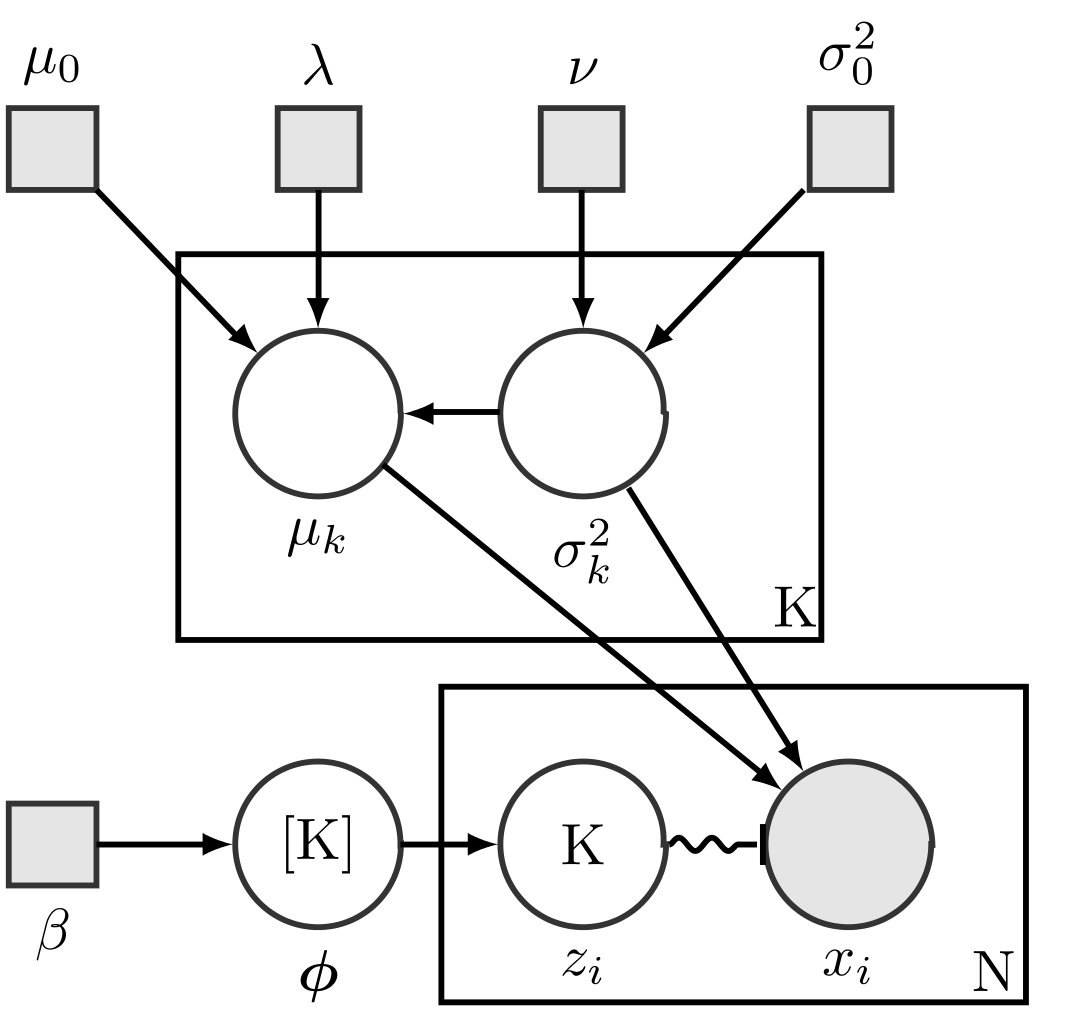
\includegraphics[height=8cm]{background/Figures/BGMM.png}
\caption{PGM representing the parametric inference of a Gaussian Mixture, see text for details. Figure by Benwing /CC BY}
\label{fig:pgmGMM}
\end{center}
\end{figure}

\section{Modelling the data}
\label{sect:datamodelling}
Creating a model is a complex task. As previously mentioned, a model is the mathematical representation of the knowledge about certain phenomenon. In this work my objective is the statistical modelling of the DANCe data related to Nearby Young Open Clusters ( NYOC), particularly the one of the Pleiades (see Section \ref{sect:DR2}).

Modelling a data set demands the gathering and arranging of the \emph{a priori} knowledge on the phenomenon. This knowledge comprises that of the data set , the NYOC: the Pleiades open cluster (Chapter \ref{chap:pleiades}), the statistical techniques that may help to attain the objective, and the computational resources at hand. I collect this knowledge from three main sources: the standard references (e.g. articles and books), my colleagues and experts on the field (\emph{knowledge elicitation}), and my self.

The structuring of the a priori knowledge and later creation the model is an iterative and continuous process.  In this Section, I describe a snapshot of this process: the state of the model once the article \citet{Olivares2017} was submitted. Later in Section \ref{sect:code}, I will give a brief description of the chronological development of the model.

In this section I will explain the statistical procedure to deal with one of the crucial aspects of the Pleiades DANCe DR2 data set: the missing values. Also, I will describe how the relevant knowledge about Pleiades cluster population and the empirical one of the field are embedded in the generative model of the data.

\subsection{Missing values}
\label{sect:missing}

Missing values refer to a non-measured or non-available (NA) value in the vector of measurements of an object. They can arise due to different statistical or physical processes. 

From the physical perspective, they occur due to faint or bright sources that produce counts values outside the dynamical range of the detector. They can also emerge due to detector malfunctions, e.g. electronic failures, or to random effects, e.g. cosmic rays. 

From the statistical perspective, important aspects of missing values are, i) the probability distribution of the sources in which they occur, and ii) if they originate due to censoring or truncation. 

In the DANCe DR2, missing values occur only in the photometric measurements (see Table \ref{tab:DR2properties}), with the bluer bands being the most affected. As expected, the probability distribution of sources with missing values is not random (uniform). Missing values occur with higher probability at the faintest and brightest ends of the photometric distributions, see Figure \ref{fig:NAsKs}. This is a crucial aspect for the statistical analysis. If missing values were randomly distributed, then, any statistical analysis derived using only objects with completely observed vectors will be unbiased. This will occur because the objects with completely observed vectors will be a random sample of the data set. Since this is not the case in the DANCe DR2, to avoid biases, objects with missing values must be incorporated in the data set and properly treated. 

\begin{figure}[ht!]
\begin{center}
%\includegraphics[width=\textwidth]{}
\caption{$K_s$ probability distribution of objects with missing values in any band except $K_s$.}
\label{fig:NAsKs}
\end{center}
\end{figure}



Truncation occurs when the data set does not contain record, nor of the measured value neither of the number of measurements, when the measured quantity lies outside certain limits. On the other hand,  censoring happens when the data set contains only partial information about the actual value of the measured quantity. Basically,  censoring happens when the value lies outside the upper or lower limits of the measuring instrument, and these limits become the only available record of the measurement. Currently, the DANCe DR2 does not provide upper or lower limits for the censored data. Although these limits could also be inferred from the data, the  heterogeneous origin of the DANCE DR2 prohibits this task. Furthermore, the missing values in the DANCE DR2 data set do not occur only because of censoring. Indeed, cosmic rays, hot pixels, halos of bright stars, diffraction patterns and cross-matching failures are just some examples of potential sources of missing values. The statistical treatment of missing values originating from all these sources lies beyond the scope of this work. However, there is a general way to deal with missing values despite their origin.

In terms of probability, there is no distinction between missing values and parameters. Therefore, we can marginalise missing values as we do with any other nuisance parameter. If the vector of measurements $\mathbf{d}$ has a missing value in entry $i$, then $x_{i} = NA$ , and $\mathbf{d}=\{x_1,x_2,...,NA,...,x_n\}$, with $n$ the dimension of $\mathbf{d}$. Thus, the marginalised likelihood of this datum, given model parameters $\mathbf{\theta}$ is

\begin{equation}
\label{eq:marginalmiss}
p(\mathbf{d}|\mathbf{\theta})= \int_{-\infty}^{\infty} p(\{x_1,x_2,...,x_{i}= NA,...,d_n\}|\mathbf{\theta})\cdot dx_{i}.
\end{equation}

Throughout this work, missing values are marginalised in this way.

%I made a remark of a point that may seem obvious but it is important to remember. Let $p(a)$ be a probability distribution, $A$ a random sample of $n$ points from it, and $p_A(a)$ the empirical probability distribution of $A$. Let $B$ be a non-random sample of $p(a)$ with $n$ elements, and empirical probability distribution $p_B(a)$. In the limit of $n\rightarrow \infty$, $p_A(a)=p(a)$ however $p_B(a)\neq p(a)$. Therefore, $p_A(a)\neq p_B(a)$. Similarly, in data with missing values, if the missing value pattern is not random, the distribution of the completely observed data (with non-missing values) differs from that of all the data. In \citet{Olivares2017} we show this subtle but important difference in the case of the DANCe data set. 

\subsection{The generative model}
\label{subsect:generative-model}
The objective of this work is the statistical study of NYOC, in particular the Pleiades cluster. Since the Pleiades data is mixed with that of the field, to achieve the objective, cluster and field populations must be disentangled. The probabilistic disentanglement of them, demands probabilistic models for each population. These models correspond to the are the field and cluster likelihoods. With these and the prior distributions, I am able to reach the objective: the posterior distributions of the parameters in the cluster model. 

In addition, cluster membership probability distributions (Eq. \ref{eq:prob}) can be computed for each object in the data set. Using these membership probability distributions together with a probability threshold, individual objects are separated into cluster and field populations.

The inference process demands a set of $N$ binary integers $\mathbf{q}$, one $q_n$ for each object. The two possible values of these binary integers represent one of the two mutually exclusive possibilities: the object belongs to the cluster ($q_n=1$) or to the field population ($q_n=0$). 

Let $\theta$ and $\phi$ be the parameters of the cluster and field models, and $p_c$ and $p_f$ their likelihoods, respectively. Then, the likelihood of the data is,

\begin{equation}
p(\mathbf{D}|\mathbf{q},\theta,\phi)= \prod_{n=1}^N {p_c(\mathbf{d}_n|\theta)}^{q_n}\cdot {p_f(\mathbf{d}_n|\phi)}^{(1-q_n)}.
\end{equation}

The inference of these $N$ binary integers will demand a computing power that is outside the current possibilities. Thus, instead of inferring them I marginalise them. 

I marginalise these $\mathbf{q}$ using a prior probability, which is set in terms of a new and unique parameter $\pi$. It represent the \emph{prior} probability that an object belongs to the field. Thus, the prior probability of $\mathbf{q}$ is

\begin{equation}
p(\mathbf{q}|\pi)= \prod_{n=1}^N {(1-\pi)}^{q_n}\cdot {\pi}^{(1-q_n)}.
\end{equation}

The marginalisation runs as

\begin{align}
p(\mathbf{D}|\pi,\theta,\phi)&=\int_{\mathbf{q}} p(\mathbf{D},\mathbf{q}|\pi,\theta,\phi)\cdot d\mathbf{q} \nonumber \\
&=\int_{\mathbf{q}} p(\mathbf{D}|\mathbf{q},\pi,\theta,\phi)\cdot p(\mathbf{q}|\pi)\cdot d\mathbf{q} \nonumber \\
&=\int_{\mathbf{q}} \prod_{n=1}^N {p_c(\mathbf{d}_n|\theta)}^{q_n}\cdot {p_f(\mathbf{d}_n|\phi)}^{(1-q_n)}\cdot \prod_{n=1}^N {(1-\pi)}^{q_n}\cdot {\pi}^{(1-q_n)}\cdot d\mathbf{q} \nonumber \\
&=\int_{\mathbf{q}} \prod_{n=1}^N \left[(1-\pi)\cdot p_c(\mathbf{d}_n|\theta)\right]^{q_n}\cdot \left[\pi\cdot p_f(\mathbf{d}_n|\phi)\right]^{(1-q_n)}\cdot d\mathbf{q} \nonumber \\
&=\prod_{n=1}^N (1-\pi)\cdot p_c(\mathbf{d}_n|\theta) + \pi\cdot p_f(\mathbf{d}_n|\phi).
\end{align}
This last equality is a rather complicated derivation which can be found on \citet{Press1997} and in \citet{Hogg2010a} for $p_c$ and $p_f$ in the exponential family. Also, a general derivation of this expression is given by \citet{Jaynes2003}. He obtains it assuming individual unknown probabilities $p_n$ instead of $q_n$ and marginalising over them by the aid of a prior.

Thus, the \emph{generative model} or likelihood of the datum $\mathbf{d_n}$  is

\begin{equation}
\label{eq:genmod}
p(\mathbf{d}_n | \pi,\boldsymbol{\theta}_c,\boldsymbol{\theta}_f,\mathbf{u}_n)=\pi \cdot p_f(\mathbf{d}_n|\boldsymbol{\theta}_f,\mathbf{u}_n) + (1-\pi)\cdot p_c(\mathbf{d}_n| \boldsymbol{\theta}_c,\mathbf{u}_n),
\end{equation}

where $\boldsymbol{\theta}_f$ and $\boldsymbol{\theta}_c$ indicate the cluster and field parameters, while $\mathbf{u}_n$ refers to the datum uncertainty. The probabilities $p_f(\mathbf{d}_n|\boldsymbol{\theta}_f,\mathbf{u}_n)$ and $p_c(\mathbf{d}_n| \boldsymbol{\theta}_c,\mathbf{u}_n)$ are the field and cluster models, respectively. These models are explained in detail in the next two sections.

In the following, I assume that the observed quantities, even if they contain missing values, resulted from the convolution\footnote{The addition of two stochastic variables is analogous to the convolution of their probability distributions.} of the \emph{true} quantities with a source of uncertainty. This last could be different for each object, thus resulting in different individual uncertainties. It means that the DANCE DR2 data is modelled allowing for its intrinsic heteroscedaticity. Although these uncertainties are not assumed to have the same values, I do assume that they have the same shape. Thus, I assume that uncertainties in our data set belong to the multivariate normal family.  This assumption is standard practice and is also supported by the large and heterogeneous origins of the DANCe DR2 data set. 

\subsection{The field population}
To model the field population, I assume that the joint seven-dimension probability distribution of the field can be factorised into the probability distributions of proper motion and photometry. Thus, the field likelihood of the proper motion and the photometry are assumed to be independent, at least conditioned on their parameters. Also, I assume that both distributions are described by Gaussian Mixture Models (GMM). The flexibility of GMM to fit a variety of distribution geometries make them a suitable model to describe the field density of the heterogeneous DANCe DR2 data. 

A GMM is a probability distribution resulting from the linear combination of $M$ gaussian distributions, $\pi_m\cdot \mathcal{N}(\boldsymbol{\mu}_m,\boldsymbol{\Sigma}_m)$, with $m=1,2,...,M$. Where $\pi_m$ is the amplitude or fraction of the $m$th gaussian. These $m$ fractions must add to one. Thus, the probability distribution resulting from a GMM is

\begin{equation}
p_{GMM}(x|\boldsymbol{\pi},\boldsymbol{\mu},\boldsymbol{\Sigma})=\sum_{m=1}^M \pi_m \cdot \mathcal{N}(\boldsymbol{\mu}_m,\boldsymbol{\Sigma}_m).
\end{equation}

Notice that the number of gaussians in the mixture is not formally speaking a parameter, but rather it implies a collection of parameters. The number of these parameters increases quadratically with the number of gaussians. 

According to \citet{Bouy2015}, the number of Pleiades candidate members in the DANCe DR2 data set is 2010 (going up to 2109 in the combined Tycho-DANCe DR2). It means that the number of field objects dominates (99.9\%) the DR2 data set. Even in our restricted $10^5$ data set, RDR2 (see Sect. \ref{sect:RDR2}), the field still dominates with a 0.98 fraction. Thus, it can be assumed that any new classification of candidate members will have a negligible impact on this figure. Therefore, it seems reasonable to assume that the GMM describing the field population can be frozen (fixed) during the process of cluster parameters inference. Let me elaborate on this assumption.

The objects that \citet{Bouy2015} classified as field are those whose cluster membership probabilities are lower than 0.75. This probability threshold corresponds to the one found by \citet{Sarro2014} after analysing the performance of their methodology when applied to synthetic data sets. In \citet{Sarro2014} the authors report that, at probability threshold $p=0.75$, the contamination and true positive rates are $\approx 8\%$ and $ \approx96\%$ respectively. Assuming that these values are correct, the number of hypothetically misclassified objects is $12\%$ of the cluster members, thus $\approx 241 $ objects. This value is negligible compared to the size of the data set ($10^5$ objects in the RDR2). It represents the negligible fraction of $ \lesssim0.0024$. 

It can be further assumed that these hypothetically misclassified objects are spread in the observables space. Indeed, these misclassified can be thought to have membership probabilities near the classification threshold. Thus, they lay in the entanglement region which corresponds, in proper motions, to a halo around the cluster centre, and in photometry, to a region around the cluster sequence.

%Furthermore, under the assumption that the work of \citet{Sarro2014} is correct, the misclassified objects concentrate on cluster membership probabilities near the classification threshold. Therefore, they will also group in an area of the physical "boundary" between the cluster and the field (I call it physical because it is on the observable variables and not in the probability threshold). This is the area of highest entanglement. It does not mean that misclassified objects will not lay in the core of the cluster (objects with high membership probabilities). It means that the occurrence of these cases will be lower.  This physical "boundary" will correspond, in proper motions space to a halo around the cluster centre. In photometry, however, this boundary will run all along the cluster sequence in the CMDs. All previous assumptions are there to justify that the negligible fraction of hypothetical misclassified  objects is not concentrated in the physical space. 

If the misclassified objects are a few and spread over the observable space, then their contribution to the parameters of the GMM describing the field population can be neglected. Thus, the parameters of the GMM remain fixed and out of the inference process. 

The previous assumption is of paramount importance due to practical reasons. If I were to simultaneously infer the parameters of both cluster and field models, the required computing time will be excessive. The number of parameters in the field GMM goes up to $\sim 300$, more than twice that of the cluster model (85 parameters). Instead, I first fit the parameters of the field GMM using the field objects in the RDR2 (the $\sim 98,000$ objects with membership probabilities below 0.75) and then I keep this parameters fixed in the inference process.   

The number of gaussians for the proper motions and photometric GMM is found using the Bayesian Information Criterion \cite[BIC,][]{Schwarz1978}. The BIC is a model selection criterium that aims at avoiding over fitting. It represents a compromise between the likelihood, $\mathcal{L}$, of the $n$ data points, and the number of parameters, $k$. This is,

\begin{equation}
\label{eq:BIC}
BIC = \ln{n}\cdot k - 2 \ln{\mathcal{L}}.
\end{equation}

To estimate the parameters of the GMM we use the Expectation Maximisation (EM) algorithm. However, the missing values in the photometry prevent the use of the standard from of the algorithm \cite[see for example Chapter 9 of][]{Bishop2006}.
Instead, I estimated these parameters with the modified version of the EM algorithm for GMM found by \citet{McMichael1996}. On this version, objects with missing values also contribute to estimate the maximum-likelihood (ML) parameters. I applied this algorithm to GMM whose number of components ranged from 1 to 20. The optimal number of gaussians suggested by the BIC is 14. 

In the case of proper motions, since they do not contain missing values, I computed the GMM parameters with the standard EM algorithm. However, the BIC favours models with large variances,  large number of components, and small fractions. Since the proper motions distribution of field objects resembles a bivariate normal, the GMM suggested by BIC was contrary to our expectations. Therefore, we decided to add a uniform distribution to the mixture of Gaussians. This uniform distribution was intended to remove the large variance and small fraction components of the GMM. I changed the EM algorithm to properly account for this modification. The BIC applied to this new mixture of distributions renders more reasonable results. This modification improves the likelihood and reduces the number of parameters. The number of gaussians suggested by the BIC for this new mixture is 7, plus the uniform distribution. 

Finally, the field likelihood $p_f(\mathbf{d}|\boldsymbol{\theta}_f,\mathbf{u})$ of an object with measurements $\mathbf{d}$, given the field parameters, $\boldsymbol{\theta}_f$,  and the standard uncertainties $\mathbf{u}$ of datum $\mathbf{d}$, is
\begin{align}
p_f(\mathbf{d}|\boldsymbol{\theta}_f,\mathbf{u})=&\left[ c\cdot\pi_{f,pm,0} + \nonumber \right. \\
&\left. \sum \limits_{i=1}^{7}\pi_{f,pm,i}\cdot \mathcal{N}(\mathbf{d}_{pm} | \boldsymbol{\mu}_{f,pm,i},\boldsymbol{\Sigma}_{f,pm,i}+\mathbf{u}_{pm})\right] \nonumber \\ 
&\cdot \left[ \sum \limits_{i=1}^{14}\pi_{f,ph,i}\cdot \mathcal{N}(\mathbf{d}_{ph} | \boldsymbol{\mu}_{f,ph,i},\boldsymbol{\Sigma}_{f,ph,i}+\mathbf{u}_{ph})\right].
\label{eq:field}
\end{align}
In this equation, $\boldsymbol{\pi}_f,\boldsymbol{\mu}_f,\boldsymbol{\Sigma}_f$ represent, respectively, the fractions, means and covariance matrices of the GMM. The first and second brackets represent the proper motion and photometric models, respectively. The first term of the proper motion model is the uniform distribution. In it, $c$ is a constant determined by the inverse of the product of the proper motions ranges (see Table \ref{tab:DR2properties}), and $\pi_{f,pm,0}$ is the fraction of this uniform distribution. The second term in the same bracket is the mixture of gaussians with means $\boldsymbol{\mu}_{f,pm}$ and covariance matrices $\boldsymbol{\Sigma}_{f,pm} +\mathbf{u}_{pm}$. 

%I refer the interested reader to Appendix \ref{appendix:A}, which contains specific details of the GMM presented in this section.

\subsection{The cluster population}
\label{subsect:cluster}
Similarly to what I assume for the field population model, I also assume that the cluster model or likelihood can be factorised in the product of the proper motions distribution times the photometric distribution. Thus, I assume these two models are independent. 

It is known that unresolved systems of stars (groups of stars that, given the spatial resolution of the telescope, are seen as an individual object) have an increased brightness proportional to the multiplicity of the system. In particular, if an unresolved system is made of two equally luminous objects, then its magnitude is 0.752 times brighter than that of an individual object. This happens on equal mass binaries.

Since the pioneer work of \citet{Trumpler1921}, we know that some of the Pleiades members are double systems. Recently, \citet{Sarro2014} show evidence that this double systems lay in an equal-mass binaries (EMB) sequence. Those authors model this displaced sequence assuming that the number of objects on it is 20\% of the total number of members. In the present work, we also model objects is this displaced EMB sequence. However, we do not assume that its proportion is fixed, we infer it from the data. 

Unresolved multiple systems, and particularly binary systems have an impact on the cluster proper motions distribution. From an astrophysical point of view, in stellar clusters, the massive objects fall towards the centre of the gravitational potential in a rate higher than that of the less massive ones. This behaviour arises from stellar encounters in which the energy exchange results in the less massive objects gaining speed and the massive ones losing it. From an astronomical point of view, an unresolved system shifts the photo centre of its images when compared to that of a single object. Given the previous considerations, we decide to model the EMB as an independent population in the proper motions. Furthermore, we pair this proper motions model to its photometric one. This more comprehensive statistical model allow us to directly compare the kinematic and photometric properties of the EBM population with those of the rest of the cluster. 

For the sake of simplicity, in the following whenever I refer to the photometric or proper motions model of the EMB I call it the EMB sequence model (with the subindex $Bs$). I refer to the model of the rest of the stars as the cluster sequence model or simply single stars. Although this is an abuse of the terminology, because there are binaries and multiple systems with different mass ratios, it keeps the text more readable.

\subsubsection{Photometric model of equal-mass binaries and single stars}

The cluster photometric sequences, both for single and EMB, are modelled with cubic splines, one for each of the $YJHK_s$ vs $CI$ CMDs. I choose the spline series due to their fitting properties. I tried several polynomial bases (Laguerre, Hermite, Chebyshev) but in spite of the order, they were not able to fit the sequence, particularly in the region around $CI \approx 3$, where the slope is higher. 

Despite their superior flexibility, spline series require more parameters than common polynomials. In addition to the coefficients of the series, they require the specification of points called knots. These knots represent the starting and ending points of the spline sections. 

Any spline function can be represented in terms of basis-splines or B-splines. By definition, a B-spline of order $n$ is a piece wise polynomial function of order $n$ in the interval $t_0 \leq x \leq t_n$. The boundary and internal points, $\mathbf{t}=\{t_0,t_1,...,t_n\}$ represent the knots. For a given set of knots, there is one and only one B-spline representation of the spline, thus the name basis spline.  In particular, any cubic spline can be represented as,

\begin{equation}
S_3(CI,\boldsymbol{\beta},\mathbf{t}) = \sum_i \beta_i\cdot B_{i,3}(CI,\mathbf{t}).
\end{equation}
Where $B_{i,n}$ are the B-splines given by the Cox-de Boor recursive formula, and $\boldsymbol{\beta}$ are the coefficients of the series. For more details on splines and the Cox-de Boor formula see \citet{deBoor1978}.



Despite their fitting properties, B-splines have an issue when inferring simultaneously their coefficients and knots: there is multi modality in the parametric space \citep{Lindstrom1999}. It means that at least more than one combination of parameters produces the same solution. To avoid this multi modality, I decided to keep the knots fixed throughout the inference. This decision, although reduces the flexibility of the splines, allows a still better fit than that of the tested polynomials. To obtain the ML estimate of the knots I use the algorithm of  \citet{Spiriti2013}. This algorithm, implemented in the \emph{freeknotsplines} R package, allows to simultaneously obtain the knots and the best truncation value for the spline series. It uses the BIC to select among compeating models. In order to obtain both the truncation of the series and the value of the knots, I use the candidate members of \citet{Bouy2015}. The BIC indicates that seven coefficients is the best number of components for the B-spline series, with the knots at $\mathbf{t}=\{0.8,3.22,3.22,5.17,8.0\}$. I tested different number of knots, ranging from two to nine, with five the best configuration given by the BIC. Since the knot at 3.22 is repeated it means that the resulting spline has lost a degree of continuity in this knot, its derivative is not continuous here.

As I mentioned in the introduction to this Section, we assume that the observed photometric quantities are drawn from a probability distribution resulting from the convolution of the observed uncertainties, with the \emph{true} quantities. Here comes an expiation. I recognise that the model is far from perfect and that there are several astrophysical phenomena that it does not addresses. Either because I do not have the knowledge or because they are too complicated to model. These phenomena include, but are not limited to, age, metallicity and distance dispersions, unresolved systems (other than EMB), variability, and transits. Instead of independently modelling each one of them, I assume that all, even those that I ignore, contribute to the model in the shape of an intrinsic photometric dispersion. Given the large and heterogeneous origins of these phenomena, we can safely assume that its total contribution has the shape of a multivariate normal distribution. The parameters of this distribution can be inferred from the data as well.

We assume that this multivariate gaussian describes both the dispersion of the cluster and EMB sequences. Most importantly, we distinguish this dispersion from the photometric uncertainty of individual measurements. If we were to assume no \emph{true} intrinsic dispersion, then any deviation from the \emph{true} quantities should have to be explained \emph{only} by the observational uncertainty. 

In our photometric model of the cluster, photometric observations are drawn from a multivariate normal distribution with five dimensions corresponding to our photometric reference set: $CI,Y,J,H,K_s$. The B-splines model the mean of the \emph{true} photometric quantities, both for the cluster sequence, $\boldsymbol{t}_{ph;Cs}$, and the EMB, $\boldsymbol{t}_{ph;Bs}$. This later one is displaced 0.75 into the bright side of the cluster sequence. The matrix, $\Sigma_{clus}$, represents the covariance matrix of the multivariate normal distribution that models the intrinsic dispersion. Covariance matrices are symmetric and positive semi-definite. Therefore, from the 25 entries in this $5\times 5$ $\Sigma_{clus}$ matrix, only 15 are unique. These are the ones we infer from the data.

Thus, the mean \emph{true} photometry is given by,

\begin{align}
\boldsymbol{t}_{ph;Cs}&= \{CI,Y,J,H,K_s\},\nonumber \\
\boldsymbol{t}_{ph;Bs}&=\{CI,Y-0.75,J-0.75,H-0.75,K_s-0.75\}, \nonumber
\end{align}
where
\begin{align}
Y &=\mathcal{S}_Y(CI,\beta_Y), \nonumber \\
J &=\mathcal{S}_J(CI,\beta_J),\nonumber \\
 H &=\mathcal{S}_H(CI,\beta_H), \nonumber \\
 K_s &=\mathcal{S}_{K_s}(CI,\beta_{K_s}),  \nonumber 
\end{align}
and $\beta_{Y,J,H,K_s}$ denote the coefficients of all the splines (a $4\times7$ matrix), which  I call $\boldsymbol{\beta}$ for the sake of simplicity.

Since the photometry of the EMB is a linear transformation, $T_{Bs}$, of the mean \emph{true} photometry of cluster sequence, no extra parameters are required. Therefore, 

\begin{align}
\boldsymbol{t}_{ph;Cs} &= \boldsymbol{\mathcal{S}}(CI, \boldsymbol{\beta}) \label{eq:trueph_Cs}\\
\boldsymbol{t}_{ph;Bs} &=T_{Bs}( \boldsymbol{\mathcal{S}}(CI, \boldsymbol{\beta})).
\label{eq:trueph_Bs}
\end{align}

Thus, cluster and EMB likelihoods of an object with photometric measurements $\mathbf{d}_{ph}$, and standard uncertainties $\mathbf{u}_{ph}$, are:
\begin{align}
\label{eq:lik-seq}
 p_{Cs}(\mathbf{d}_{ph}| CI, \boldsymbol{\beta},\Sigma_{clus},\mathbf{u}_{ph})={\mathcal{N}}(\mathbf{d}_{ph}|\boldsymbol{t}_{ph;Cs}, \mathbf{u}_{ph}+\Sigma_{clus}),\nonumber \\
p_{Bs}(\mathbf{d}_{ph}| CI, \boldsymbol{\beta},\Sigma_{clus}, \mathbf{u}_{ph})={\mathcal{N}}(\mathbf{d}_{ph}|\boldsymbol{t}_{ph;Bs}, \mathbf{u}_{ph}+\Sigma_{clus}),
\end{align}
where $\boldsymbol{t}_{ph;Cs}$ and $\boldsymbol{t}_{ph;Bs}$ are given by Equations \ref{eq:trueph_Cs} and \ref{eq:trueph_Bs}, respectively.

Since the splines are parametrised by the true $CI$ of each object, we have more parameters than objects in our data set \footnote{Although this sounds crazy, the rules of probability calculus do not discard this possibility.}. This \emph{true} $CI$ is unknown even if its observed value is not missing. We solve this problem (it is a computational problem!) by marginalising these nuisance parameters (See Eq. \ref{eq:clmarginalps} and \ref{eq:clmarginalpb}). 

To marginalise these $CI$s we need a prior, which we provide in a hierarchical way (thus the name Bayesian Hierarchical model). This marginalisation leaves behind a precise estimate of the parameters of the prior distribution. Paradoxically, all objects, even those without a measurement of the $CI$ contribute to this estimate. Here lays the force of the BHM.

We model the prior of the \emph{true} $CI$ as a truncated ($0.8\leq CI \leq8$) univariate GMM with five components, whose parameters are also inferred from the data. We chose five components as suggested by BIC. I applied BIC to the results found using the standard EM algorithm for univariate GMM applied to the candidate members of \citet{Bouy2015}. I tested with larger number of components in the mixture, but the posterior distribution did not changed, thus indicating that the BIC value was a proper assumption.

 Thus, the GMM modelling the prior of the \emph{true} $CI$ is 

\begin{equation}
\label{eq:colordist}
p_{CI}(CI|\boldsymbol{\pi}_{CI},\boldsymbol{\mu}_{CI},\boldsymbol{\sigma}_{CI})= \sum_{i=1}^5 \pi_{CI,i} \cdot \mathcal{N}_t(CI| \mu_{CI,i},\sigma_{CI,i}).
\end{equation}

In this last Equation, the symbol $\mathcal{N}_t$ stands for the truncated ($0.8<CI<8$) univariate normal distribution.

Then, the marginalisation of $CI$ runs as follows:
\begin{align}
\label{eq:clmarginalps}
 p_{Cs}(\mathbf{d}_{ph}| \boldsymbol{\theta}_c,\mathbf{u}_{ph})&=\int p_{Cs}(\mathbf{d}_{ph},CI| \boldsymbol{\theta}_c,\mathbf{u}_{ph}) \cdot dCI \nonumber \\
 &=\int p_{Cs}(\mathbf{d}_{ph}|CI, \boldsymbol{\theta}_c,\mathbf{u}_{ph}) \cdot p_{Cs}(CI| \boldsymbol{\theta}_c,\mathbf{u}_{ph})\cdot dCI 
\end{align}
\begin{align}
\label{eq:clmarginalpb}
p_{Bs}(\mathbf{d}_{ph}| \boldsymbol{\theta}_c,\mathbf{u}_{ph})&=\int p_{Bs}(\mathbf{d}_{ph},CI| \boldsymbol{\theta}_c,\mathbf{u}_{ph})\cdot dCI \nonumber \\
 &=\int p_{Bs}(\mathbf{d}_{ph}|CI, \boldsymbol{\theta}_c,\mathbf{u}_{ph})\cdot p_{Bs}(CI| \boldsymbol{\theta}_c,\mathbf{u}_{ph})\cdot dCI.
\end{align}
In these Equations, $\theta_c$ stands for all cluster parameters related to photometry, and the first and second terms of the integrals in the last equalities correspond to Equations \ref{eq:lik-seq} and \ref{eq:colordist}, respectively. The distribution of $CI$ depends only on $\boldsymbol{\pi}_{CI},\boldsymbol{\mu}_{CI},\boldsymbol{\sigma}_{CI}$, thus, the cluster and equal-mass binaries likelihoods of datum $\mathbf{d}_{ph}$ are 
\begin{align}
\label{eq:lik-seq2}
 &p_{Cs}(\mathbf{d}_{ph}|\boldsymbol{\pi}_{CI},\boldsymbol{\mu}_{CI},\boldsymbol{\sigma}_{CI},\boldsymbol{\beta},\Sigma_{clus},\mathbf{u}_{ph}) \nonumber \\
 &=\int{\mathcal{N}}(\mathbf{d}_{ph}|\boldsymbol{\mathcal{S}}(CI, \boldsymbol{\beta}), \mathbf{u}_{ph}+\Sigma_{clus}) \nonumber \\
 &\cdot \sum_{i=1}^5 \pi_{CI,i}\cdot \mathcal{N}_t(CI| \mu_{CI,i},\sigma_{CI,i}) \cdot dCI\nonumber \\
&p_{Bs}(\mathbf{d}_{ph}|\boldsymbol{\pi}_{CI},\boldsymbol{\mu}_{CI},\boldsymbol{\sigma}_{CI}, \boldsymbol{\beta},\Sigma_{clus}, \mathbf{u}_{ph})\nonumber \\
&=\int{\mathcal{N}}(\mathbf{d}_{ph}|T_{Bs}( \boldsymbol{\mathcal{S}}(CI, \boldsymbol{\beta})), \mathbf{u}_{ph}+\Sigma_{clus}) \nonumber \\ &\cdot \sum_{i=1}^5 \pi_{CI,i}\cdot \mathcal{N}_t(CI| \mu_{CI,i},\sigma_{CI,i}) \cdot dCI.
\end{align}

The observed $CI$ and magnitudes help us  to reduce the computing time of the marginalisation integral. We use them to discard  regions of the integral in which the argument is almost zero (i.e. far from the measured values). Although we allow the nuisance parameters $CI$s to have all their possible values, the data, by means of the likelihood, give us information about the distribution of these individual nuisance parameters. To use this information, we proceed as follows. First, we compare the observed photometry to the true one (i.e. the cluster sequence given by the splines). For it we use a grid of 300 points uniformly distributed in the domain of $CI$ ($0.8<CI<8$). Then, we find the point, $p$, of the grid that is  the closest to the vector of the observed photometry.  Distance is computed under  the Mahalanobis metric. This metric takes into account the observational uncertainty, $\mathbf{u}_{ph}$, and the intrinsic dispersion of the cluster sequence, $\Sigma_{clus}$. Finally, the limits of the marginalisation integral  are defined as those given by a ball of 3.5 Mahalanobis distances around point $p$. Contributions outside this ball are negligible to the integral ($< 4\times10^{-4}$).

\subsubsection{Proper motion model of equal-mass binaries and single stars}
As mentioned before, we assume that the cluster population has two subpopulations: single and EMB stars.
We model the proper motions of these two subpopulations with independent GMM. If the cluster is virialised (see Chapter \ref{chap:pleiades}), we can assume that its velocity distribution is almost Maxwellian (Maxwell-Boltzman distribution). Therefore a GMM is a reasonable assumption. Furthermore, in the absence of external forces, a virialised system is expected to have spherical symmetry both in its spatial and velocity distributions. Thus we can safely assume that the gaussians within each GMM are concentric, thus they share the same mean. However we allow independent means for both single and EMB subpopulations. The assumption of spherical symmetry may be a weak one in the presence of the galactic potential. It can perturb the cluster and deviate its spatial and velocity distribution from spherical symmetry. Furthermore, the ellipticity of the spatial distribution, which has been reported to be no negligible \cite[$\epsilon=0.17$, according to ][]{Raboud1998}, can due to projection effects further deviate the observed velocity distribution profile from spherical symmetry. Nevertheless, since we model the covariance matrices of the GMM of both single and EMB, as full covariance matrices, any departure from the spherical symmetry in the velocity distribution can still be perfectly modelled by the non diagonal entries of these matrices.


We infer the parameters of these GMMs as part of our Bayesian hierarchical model. However we a priori set the number of gaussians in each GMM. Not doing so will demand a technique in which the model parameters can be augmented. Although such techniques already exist, they are still under computational development \cite[see][for a review of reversible jump MCMC]{Fan2011}.

Using the EM for GMM and the proper motions of the candidate members of \citet{Bouy2015}, I obtained the ML estimates for the GMM likelihoods. I did this for configurations of GMM ranging from one to five components. The BIC (Eq. \ref{eq:BIC}) suggested four and two gaussians for cluster and EMB GMM, respectively. Since covariance matrices are always symmetric, only three parameters are needed to fully specify the covariance matrices of these bivariate normal distributions.

Thus, the cluster (subindex $Cs$) and EMB (subindex $Bs$) likelihoods of an object with proper motions measurements $\mathbf{d}_{pm}$, and uncertainties $\mathbf{u}_{pm}$, are

\begin{align}
p_{Cs}(\mathbf{d}_{pm}| \boldsymbol{\pi}_{Cs}, \boldsymbol{\mu}_{Cs},\boldsymbol{\Sigma}_{Cs},\mathbf{u}_{pm})
&= \sum_{i=1}^4\pi_{Cs,i}\cdot \mathcal{N}(\mathbf{d}_{pm} | \boldsymbol{\mu}_{Cs},\Sigma_{Cs,i}+\mathbf{u}_{pm}) \nonumber\\
p_{Bs}(\mathbf{d}_{pm}| \boldsymbol{\pi}_{Bs}, \boldsymbol{\mu}_{Bs},\boldsymbol{\Sigma}_{Bs},\mathbf{u}_{pm})
&= \sum_{i=1}^2\pi_{Bs,i}\cdot \mathcal{N}(\mathbf{d}_{pm} | \boldsymbol{\mu}_{Bs},\Sigma_{Bs,i}+\mathbf{u}_{pm}).
\label{eq:lik-pm}
\end{align}

Finally, combining the proper motions and photometric models, the total cluster likelihood of an object with measurement $\mathbf{d}$, and uncertainties $\mathbf{u}$, is

\begin{align}
p_c(\mathbf{d}|\boldsymbol{\theta}_c,\mathbf{u})&=\pi_{CB}\cdot p_{Cs}(\mathbf{d}_{pm}| \boldsymbol{\pi}_{Cs}, \boldsymbol{\mu}_{Cs},\boldsymbol{\Sigma}_{Cs},\mathbf{u}_{pm}) \nonumber \\ &\cdot  p_{Cs}(\mathbf{d}_{ph}|\boldsymbol{\pi}_{CI},\boldsymbol{\mu}_{CI},\boldsymbol{\sigma}_{CI},\boldsymbol{\beta},\Sigma_{clus},\mathbf{u}_{ph})\nonumber\\
&+(1-\pi_{CB})\cdot p_{Bs}(\mathbf{d}_{pm}| \boldsymbol{\pi}_{Bs}, \boldsymbol{\mu}_{Bs},\boldsymbol{\Sigma}_{Bs},\mathbf{u}_{pm}) \nonumber \\
&\cdot  p_{Bs}(\mathbf{d}_{ph}|\boldsymbol{\pi}_{CI},\boldsymbol{\mu}_{CI},\boldsymbol{\sigma}_{CI}, \boldsymbol{\beta},\Sigma_{clus}, \mathbf{u}_{ph}),
\end{align}

where $\pi_{CB}$ is the parameter representing the amplitude of single cluster sequence stars in the single-EMB mixture model. The photometric and proper motions likelihoods are given by Equations \ref{eq:lik-seq2} and \ref{eq:lik-pm}, respectively.
 
\section{Priors}
\label{sect:priors}
The Bayesian formalism is characterised by the use of priors. These priors, as mentioned earlier, represent the objective (measurable and reproducible) way to establish beliefs about the distribution of values that certain parameter may have. 

In the following I describe the information used to establish both the family of the prior distribution as well as its hyperparameters. The priors we assume are intended to fall, in most of the cases, in the category of weakly informative priors. A weakly informative prior provides weaker information than the one actually available \citet{Gelman2006}. This kind of priors show better computational performance when compared to non-informative priors. Examples of these can be found in the works of \citet{Gelman2008} and \citet{Chung2015}. 

I group priors into three main categories. Fractions in general, and those concerning: proper motions and photometric models. 

Fractions are defined for mixtures. The mixtures in the model are the GMMs, the cluster-field, and the single-EMB mixtures. At each mixture, the fractions or amplitudes quantify the contribution of each element to the mixture. If each element in the mixture is itself a probability distribution, then the fractions must add to one and be bounded by the $[0,1]$ interval. We choose the Dirichlet distribution since it is the multivariate generalisation of the beta distribution. It has support in $[0,1]$ for each entry, and is parametrised by $\boldsymbol{\alpha}$. This distribution gives the probability of $n$ rival events given that each rival event has been observed $\alpha_i-1$ times ($i=\{1,2,...,n\}$).

The mean and variance of the Dirichlet distribution are given by,

\begin{equation}
E[x_k]=\frac{\alpha_k}{\sum_k \alpha_k},
\end{equation}

\begin{equation}
Var[x_k]=\frac{-\alpha_k\cdot (\alpha_k -\sum_k \alpha_k)}{(\sum_k \alpha_k)^2 \cdot (1+\sum_k \alpha_k)}.
\end{equation}

For the field-cluster mixture we set the hyper-parameters to $\boldsymbol{\alpha}=\{9.8,0.2\}$. We expect a mean 98\% of field objects and a 2\% of cluster objects with little variance. These figures correspond to the fraction of field and cluster candidate members found by \citet{Bouy2015}. 
For the single-EMB mixture we use an hyper-parameter value, $\boldsymbol{\alpha}_{CB}=\{8,2\}$. We expect a mean 20\% of EMB, as suggested by \citet{Bouy2015}. 
For fractions in the proper motions GMM, hyper-parameter are $\boldsymbol{\alpha}_{Cs}=\{1,1,5,5\}$ and $\boldsymbol{\alpha}_{Bs}=\{1.2,8.8\}$. These values induce fraction distributions whose means are similar to the fractions recovered after fitting a GMM to the \citet{Bouy2015} candidate members. 
For the fraction in the GMM of the $CI$ distribution, the hyper-parameter were set all to 1, ($\boldsymbol{\alpha}_{CI}=\{1,1,1,1,1\}$), which results in equal means and large variances for all of them.

In the previous cases, with exception of the cluster-field mixture, the hyper parameters were chosen to have larger variances. Fig.  \ref{figure:priors} shows the distribution associated to these hyper-parameters.

The narrow variance in the cluster-field mixture expresses our prior belief about the number (fraction) of candidate members within our large data set. I believe this figure is small.

\begin{figure*}[htbp]
\begin{center}
%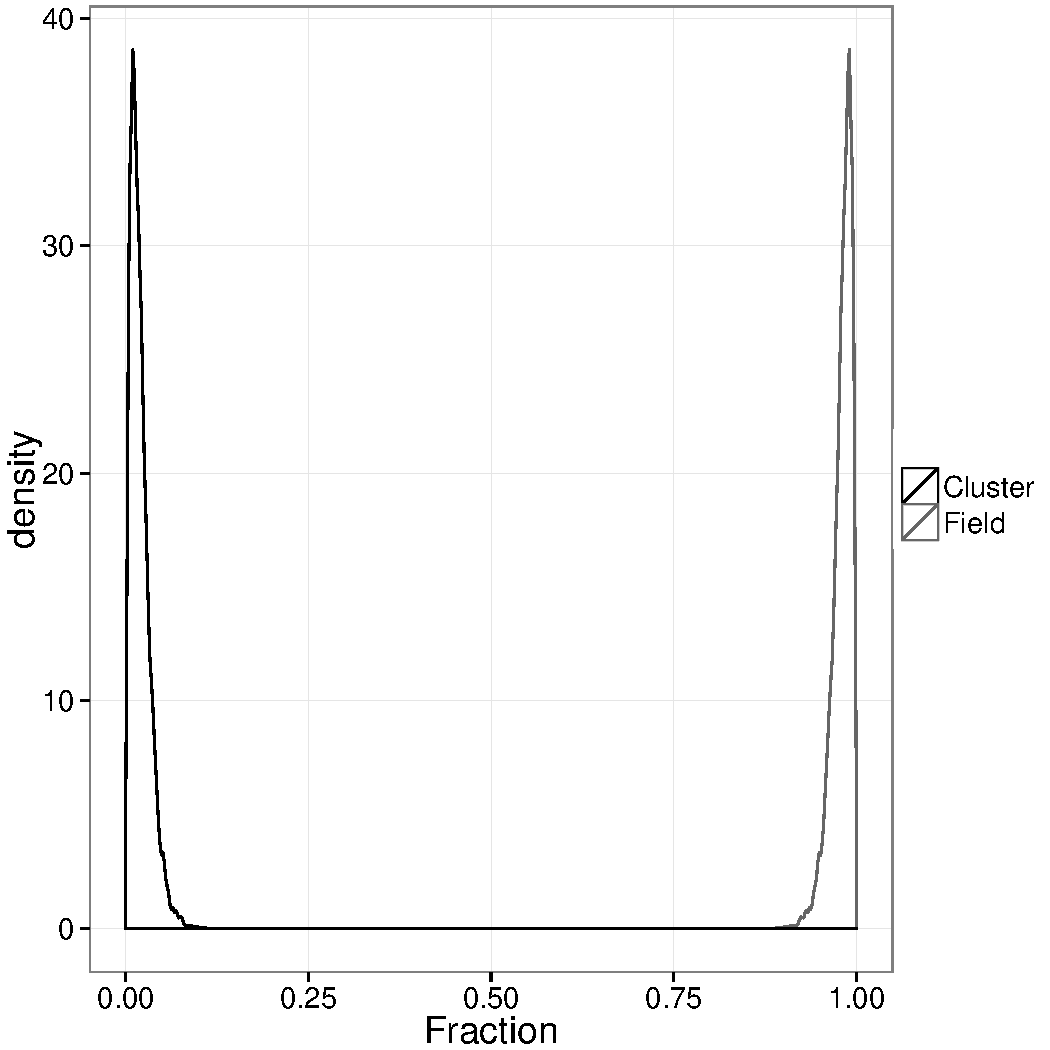
\includegraphics[page=1,width=8cm]{figs/priors.pdf}
%\includegraphics[page=2,width=8cm]{figs/priors.pdf}\\
%\includegraphics[page=3,width=8cm]{figs/priors.pdf}
%\includegraphics[page=4,width=8cm]{figs/priors.pdf}
\caption{Prior distribution of fraction parameters. From top left to bottom right, the distributions of field fraction ($\pi$), equal mass binaries fraction ($1-\pi_{CB}$), and the cluster ($\pi_{Cs}$) and equal-mass binaries ($\pi_{Bs}$) fractions in their proper motion GMM, respectively.}
\label{figure:priors}
\end{center}
\end{figure*}


For the priors of mean parameters in the proper motions GMM, both of single and EMB, we choose the bivariate normal distribution. We set the hyper-parameters of this bivariate normal to the MLE found after fitting a bivariate normal to the candidate members of \citet{Bouy2015}. These values are $\boldsymbol{\mu}_{\mu_{pm}}=\{16.30,-39.62\}$ and $\Sigma_{\mu_{pm}}=\{\{36.84,1.18\},\{1.18,40.71\}\}$. 

As prior for the covariance matrices of both single and EMB proper motions GMM we use the Half--$t(\nu,\mathbf{A})$ distribution. With $\nu$ an scalar and $\mathbf{A}$ a vector of dimension equal to that of the space. As shown by \citet{Huang2013} this family distribution leads to more accurate estimation of covariance matrices than the traditional Inverse-Wishart distribution. Particularly, the marginal correlation correlation parameters, $\rho$ have the following distribution,

\begin{equation}
p(\rho) \propto (1-\rho^2)^{\frac{\nu}{2}-1}
\end{equation}
while the standard deviation term $\sigma_k$ associated to entry $k$ is distributed according to Half--$t(\nu,A_k)$. We set the hyper-parameter to $\nu=3$ and $\boldsymbol{A}_{pm}=\{10^5,10^5\}$. According to \citet{Huang2013}, an arbitrarily large values of $\boldsymbol{A}$ lead to arbitrarily weakly informative priors on the corresponding standard deviation terms.

Photometric priors can be grouped in three categories, those concerning: (i) the \emph{true} $CI$, (ii) the splines coefficients, and (iii) the cluster sequence intrinsic dispersion. 

For the means in the univariate GMM modelling $CI$ we use a uniform in the range  ($0.8\leq CI \leq8$). For the standard deviations I choose the Half--Cauchy$(0,\eta)$ distributions as suggested by \citet{Gelman2006}. I choose the arbitrarily large value of $\eta=100$..

\sloppy
For the coefficients in the spline series we set the priors as univariate normal distributions. To find the values of the hyper-parameters, we proceed as follows. First, we remove EMB from \citet{Bouy2015} candidate members. I performed an iterative fit of the cluster sequence, such that in each iteration objects above the 0.75 magnitude were removed. In the region of $CI > 7$ no candidate members have been found. Thus, to provide a prior we complement our list of candidate members with the brown-dwarfs from the \citet{Faherty2012} sample. Only those with the same CMD as our data set. Finally, we fit the splines, and use the coefficients of this fit as means, $\mu_{\beta}$ of the univariate normal distributions. The standard deviation terms were set to $\sigma_{\beta}=\{1,1,1,1,1,0.5,0.1\}$. These values provide a reasonable compromise between cluster sequences compatible with the previously known candidates and those far away or with exotic shapes. We show a sample of this priors in Fig. \ref{figure:priorcoefs}. This Fig. also shows the brown-dwarfs from \citet{Faherty2012} and the sequence (dashed line) we use to provide the means of the univariate normal distributions.

To set the prior for the parameters of the cluster intrinsic dispersion, I choose again the Half--t$(\nu,\boldsymbol{A})$ distribution.  However, this time I use  $\boldsymbol{A}_{ph}=\{10,10,10,10,10\}$. These values are large when compared to the standard deviation terms o the observation uncertainty, thus provide a weakly informative prior on the marginal standard deviation terms of the $\Sigma_{clus}$ covariance matrix.

Table \ref{table:hyperparameters} shows a summary all the hyper-parameter and their values.

%\input{figs/HyperParameters.txt}

\begin{figure}[htbp]
\begin{center}
%\resizebox{\hsize}{!}{\includegraphics[page=4]{figs/Priors_Coefs.pdf}}
\caption{CMD $K_s$ vs. $i-K_s$ showing a sample of the prior for the coefficients in the splines series. Also shown the brown-dwarfs we add from \citet{Faherty2012} sample, and the cluster sequence (dashed line) found after fitting the splines to the brown-dwarfs and candidate members below the equal-mass binaries sequence.}
\label{figure:priorcoefs}
\end{center}
\end{figure}

%\input{figs/SymbolParameters.txt}

\section{Sampling the posterior distribution}
Theoretically, there are at least three possible approaches to obtain the posterior distributions of the parameters in our model. One of these theoretical options is the analytical solution. This solution is obviously not feasible, due to our large data set. The second theoretical option consists of a grid in parameter space. The likelihood and the prior must be evaluated at each point in this grid and then multiplied. This approach is reasonable when the parametric space is of moderate dimension. It requires the evaluation of the posterior distribution $q^p$ times, with $q$ the number of grid points in one dimension, and $p$ the dimension of the parametric space. The number of parameters in our model is 85, which immediately rules out this possibility. The third and so far only feasible approach is the use of Markov Chain Monte Carlo (MCMC). Although these methods provide a solution in a reasonable time, nevertheless, the bottle neck of computing time is due to the evaluation of the likelihood, which rows linearly with the size of the data set. 

This Section is structured as follows. First, I introduce an heuristic technique to search for the maximum a posteriori of our target distribution: the posterior distribution of the parameters given the data. Then I will describe the MCMC techniques available in the literature. Particularly the one we chose and the reasons for which it was chosen. I will end this section with the details about the assessment of the MCMC convergence.

\subsection{PSO}

The likelihood of the data is the product of the individual likelihoods of each datum (Eq. \ref{eq:lik_datum}). Therefore, the number of operations needed to evaluate the likelihood grows proportionally to the size of the data set. As I will explain in Section \ref{sect:MCMC}, the burn-in phase of MCMC techniques allows them to reach the target distribution. However, once the MCMC reaches the target distribution, the burn-in computations are discarded. Since the evaluation of the likelihood, and therefore of the posterior, is computationally expensive due to our large data set, I decided to reduce as much as possible the burn-in phase. To do so, I provide MCMC with a set of initial solutions which are close to the Maximum-A-Posteriori (MAP) of the target (posterior) distribution. These MAP solution must not be crowded on the MAP solution, otherwise MCMC will spend a lot of time in expanding this initial set of solutions.  Our objective is a representative sample of the full posterior distribution, not just an estimate of it.

In Section \ref{sect:MCMC}, I will show that the MCMC flavour more suitable to our objective belongs to the family of \emph{ensemble} MCMC. This flavour works with particles in the parametric space. To make the transition between the initial MAP solutions and the particle MCMC as efficient as possible I chose a MAP finder which works also with particles. The Particle Swarm Optimiser \cite[PSO,][]{Kennedy1995} provides a heuristic cheap and fast approach to the MAP solution. The PSO works with an ensemble of particles which move in through the parametric space. These particles use the collective and individual past and present information to update their position. This information is specified by the score function, which in our case is the posterior distribution. The particles update their position iteratively by means of a velocity. It has a random but restricted magnitude, however, its direction is determined by the object position and the individual and collective positions of maximum score. \citet{Kennedy1995} has a detailed description of the original algorithm, while a more efficient version is given by \citep{Clerc2002}.

Although the PSO is a simple and rather efficient solution to the MAP approximation, it is far from perfect. Due to its heuristic origin, there is no theory behind its formulation, furthermore, it does not always guarantee the finding of the global maxima. A convergence guaranteed version can be found in \citet{Patel2013}. This issue does not affect our results because MCMC does guarantee the target distribution. However, it has an impact in the computing time. Also, PSO stops once the particles scores are within a user defined tolerance. If the tolerance is too large, the PSO may not converge. If the tolerance is small it may converge but deliver solutions highly concentrated around the solution. This poses a problem to the following MCMC stage. In order to explore the full posterior distribution MCMC needs more iterations to expand the initially concentrated positions. To overcome this problem I decided to use the charged PSO \citep{Blackwell2002}


\subsubsection{The charged PSO}
Originally designed to optimise a time varying score function, the charged PSO maintain its exploratory capabilities due to an electrostatic force that repels particles when they got closer than a certain distance \citep{Blackwell2002}. Thanks to this electrostatic force the charged PSO avoids the over-crowding of particles around local best values.

The algorithm of \citet{Blackwell2002} computes distances in the entire parametric space. I find this approach unsuitable to our problem, thus I modified it. This modified version is described in more details on Section \ref{sect:chargedPSO}. 

 
\subsection{MCMC}
\label{sect:MCMC}
\subsubsection{Generalities}
Markov chain Monte Carlo is the generic name for a series of algorithms whose objective is the sampling of probability distributions. As their name indicates, MCMC generate a chain of Monte Carlo realisations that fulfil the Markov property. Monte Carlo realisations can be understood, broadly speaking as continuous random realisations. Since it is an iterative algorithm, the chain refers to the joint of al random Monte Carlo steps. The Markov property refers to the probabilistic independence of the steps in the chain. A Markov chain is that in which the probability of a future step depends only on the present step, and not in the past steps.

\citet{Andrieu2003} provides a brief and interesting summary of the history of the MCMC methods. In the following I use their work to describe the fundaments of MCMC. For more details, see the aforementioned authors and the book of \citet{Brooks2011}.

A stochastic process is defined as a sequence  $\{\theta_1,...,\theta_n\}$ of random elements from a set, where each element $\theta_i \subset \mathbb{R}^k$  with $k$ the dimension of the \emph{state space}. 

A stochastic process, $\boldsymbol{\theta}=\{\theta_0,\theta_1,...,\theta_n,\theta_{n+1}\}$ is called a Markov chain if
\begin{equation}
p(\theta_{n+1} | \theta_0,\theta_1,...\theta_n) = p(\theta_{n+1} |\theta_n). \nonumber
\end{equation}

A Markov chain has two important distributions, the initial distribution and the transition distribution. The initial distribution is the marginal distribution of $\theta_0$, it is $p(\theta_0)$. The transition distribution is the conditional probability $p(\theta_{n+1} |\theta_n)$. This last one is called stationary or homogeneous if it does not depend on $n$.

If this transition is irreducible and aperiodic, then there is an invariant or equilibrium distribution to which the chain converge in spite of the initial distribution. Aperiodic means that the chain does not make loops. It is irreducible if the probability of exploring all other states is not zero.

If we want to have $p(\theta)$ as the invariant distribution, then it suffices that the transition distribution $p_t(\cdot | \cdot)$ satisfies the detailed balance condition,
\begin{equation}
p(\theta_{n})\cdot p_t(\theta_{n-1}|\theta_n)=p(\theta_{n-1})\cdot p_t(\theta_n | \theta_{n-1})
\end{equation}

Thus MCMC are Markov chains that satisfy the detailed balance and had their invariant distribution as the target distribution. 
The variety of MCMC algorithms arises from the efficiencies in which they arrive to the target distribution.

In the following I will review three of the MCMC categories: Metropolis-Hasting (MH), Hamiltonian Monte Carlo (HMC), and affine invariant samplers. The MH category comprises the classic MH algorithm but also contain particular cases like the Gibbs sampler \citep{Geman1984}. I describe MH only for completeness and explanatory reasons. Later, I will focus on the particular cases of Hamiltonian Monte Carlo, for (HMC), affine invariant for ensemble samplers. Finally, I will briefly describe Nested Sampling, an algorithm that uses MCMC to numerically compute the Bayesian evidence while simultaneously samples the posterior distribution. 
\subsubsection{Metropolis-Hastings}
By far, the most popular MCMC algorithm is Metropolis-Hastings \citep{Metropolis1953,Hastings1970}. Given the current, $\theta$, and proposed, $\hat{\theta}$ positions of the Markov chain, which live in the state space, the chain moves from $\theta$ to $\hat{\theta}$ with acceptance probability

\begin{equation}
\mathcal{A}(\hat{\theta}|\theta)=min\left\{1,\frac{p(\hat{\theta})\cdot q(\theta|\hat{\theta})}{p(\theta)\cdot g(\hat{\theta}|\theta)}\right\}.
\end{equation}
Where $q$ is the transition probability. Since the algorithm allows rejection, it is aperiodic, and to ensure irreducibility, the support of $q$ must include that of $p$ \citep{Andrieu2003}. The popularity of MH lies in its simplicity. Nevertheless it requires a careful tuning of the transition probability. 

\subsubsection{Hamiltonian Monte Calro}
The Hamiltonian Monte Carlo algorithms \citep{Duane1987,Neal1996}, as they name suggests\footnote{Originally called Hybrid Monte Carlo by \citep{Duane1987}}, use Hamiltonian dynamics to express the target distribution as the potential distribution of a hamiltonian system. In such systems total energy is the sum of the potential and kinetic energies. The potential distribution depends only on position, whereas the kinetic one on momentum. To this end, HMC introduces a momentum to fictitious particles to use their positions as a sample of the target distribution. To update the particles positions, HMC uses the Hamilton equations. They contain information about the gradient of the potential. Once HMC has tuned the momentum distribution, the proposed positions are more likely in terms of the target distribution. Therefore, using the information about the gradient of the target distribution, HMC is able to improve the acceptance ratio of the proposed steps. A detailed description of HMC can be found in Chapter 5 of \citet{Brooks2011}. The package \emph{Stan} \citep{Stan} provides an efficient implementation of HMC.

\subsubsection{Affine invariant}
Affine invariant MCMC samplers use many particles, (ensemble), to sample the target distribution with a performance that is independent of its shape in the parametric space. Affine invariant MCMC do not need to tune the transition distribution, for this reason, these samplers are faster than standard MCMC \citep{Goodman2010}. In the following I use the derivation of \citet{Goodman2010}.


An ensemble $\boldsymbol{\theta}$ is a set of $L$ particles $\theta_l \subset \mathbb{R}^k$ living in state space $\mathbb{R}^{kL}$. These particles are independently drawn from the target distribution $\pi$. Therefore,

\begin{equation}
\Pi(\boldsymbol{\theta})=\pi(\theta_1)\cdot\pi(\theta_2)...\pi(\theta_L).\nonumber 
\end{equation}

Thus, an ensemble MCMC is a Markov chain in the state space of ensembles, more properly, in the state space of the sequence $\boldsymbol{\theta}(1),\boldsymbol{\theta}_(2),...\boldsymbol{\theta}(t)$. An ensemble MCMC preserves the equilibrium distribution without the individual particles sequence, $\theta_1(1),\theta_1(2),...\theta_1(t)$, being Markov or even independent.

To update the particles positions, the detailed balance must be fulfilled. \citet{Goodman2010} use partial resampling to ensure this. The transition preserves the target distribution if the single particle move preserves the conditional distribution of the particle given the complementary ensemble (the rest of the particles). Using the affine invariant \emph{stretch move}, they are able to define a Markov chain (in the state space of ensembles) that satisfies the detailed balance. The stretch move $\theta_k(t) \rightarrow \hat{\theta}$, defined as,
\begin{equation}
\label{eq:stretchmove}
\hat{\theta}= \theta_j(t) + z\cdot(\theta_k(t)-\theta_j(t)),\nonumber 
\end{equation}
where $\theta_j(t)$ is the current position of a particle in the complementary ensemble, and $z$ is the stretching factor. It produces a symmetric transition, $p(\theta_k(t) \rightarrow \hat{\theta})=p(\theta_k(t) \leftarrow \hat{\theta})$, if its density $g(z)$ satisfies the symmetry condition
\begin{equation}
g(\frac{1}{z})= z\cdot g(z).\nonumber 
\end{equation}
Finally, \citet{Goodman2010} define their affine invariant MCMC using $g(z) \propto 1/z, z\in[1/a,a]$ and zero otherwise, together with acceptance probability,

\begin{equation}
\mathcal{A}(\hat{\theta}|\theta)=min\left\{1,z^{n-1}\cdot \frac{p(\hat{\theta})}{p(\theta)}\right\}.
\end{equation}
The parameter $a>1$ improve the performance the performance of the sampler  \citep{Goodman2010}.

One of the greatest advantages of  ensemble samplers is its possibility of parallelisation. Since they work with particles, this particles can be distributed among cores in a computer cluster, therefore reducing considerably the computing time. \citet{Foreman2013} implemented the affine invariant stretch move of \citet{Goodman2010} in the Python package \emph{emcee}. 
\subsubsection{Nested sampling}
Nested sampling \citep{Skilling2004,Skilling2006} is an algorithm designed to numerically integrate the evidence (Eq. \ref{eq:evidence2}). As a by product it delivers also a sample of the posterior distribution. It samples the prior and use these particles to compute integral. The integral is the sum of the likelihood, $L_i$ of each particle times a weight, $w_i$. This weight is a proxy of the volume of the prior covered by the updated position of the particle, $w_i = \exp(-(i-1)/N) - \exp(-i/N)$. Particles update their position only when their likelihood is the minimum from the group of particles. In this way,

\begin{equation}
z \leftarrow \sum_i w_i\cdot L_i
\end{equation}

An improved version of the original algorithm was implemented in \emph{MultiNest} \citep{Feroz2009}. This version allows the sampling and computing of evidence in multimodal posteriors.

\subsubsection{Implementation and convergence}
To sample the posterior distribution in our problem, we chose \emph{emcee} due to the following properties: i) the affine invariance allows a faster convergence over common and skewed distributions \cite[see][for detail]{Goodman2010,Foreman2013}, ii) the parallel computation distributes particles over nodes of a computer cluster and thus reduces considerably the computing time, and iii) it requires the hand-tuning of only two constants: the number of particles, and the parameter $a$ of the $g(z)$ distribution. I choose a particle to parameters ratio of two, this means 170 particles. This is the minimum recommended by \citet{Foreman2013} that allows a reasonable computing time. After trial and error, I fixed the value of parameter $a=1.3$. As mentioned by \citet{Goodman2010} this parameter can be tuned to improve performance of the sampler. The chosen value keeps the acceptance fraction in the range $0.2-0.5$ as suggested by \citet{Foreman2013}.

I use a modified version of \emph{CosmoHammer} \citep{Akeret2013}, a front-end of \emph{emcee}. See section \ref{sect:HHPC} for more details. 

As mentioned earlier, the PSO does not guarantee the finding of the global maximum of the score function. Therefore, I decide to implement an iterative approach that minimises the risk of PSO to get stuck in a local maxima. To do so I iteratively run PSO and 50 iterations of \emph{emcee} (with the same number of particles as the PSO) until the relative difference between means of consecutive iterations was lower than $10^{-7}$. The iterations of \emph{emcee} spread the PSO solution without moving away from the maximum. 
 
Neither scheme, PSO alone or PSO-\emph{emcee}, guarantees to find the global maximum and their solution could be biased. However, we use them to obtain a fast estimate of the global maximum, or at least, of points in its vicinity. If the initial solution provided by this scheme is indeed biased, the final \emph{emcee} run, during the burning phase, erases any dependance on these initial solutions. After convergence of the PSO-\emph{emcee} scheme, we run \emph{emcee} until convergence.  
 
Convergence to the target distribution occurs when each parameter enters into the stationary equilibrium, or normal state. The Central Limit Theorem ensures that this state exists. See \citet{Roberts2004} for guaranteeing conditions and \citet{Goodman2010} for \emph{irreducibility} of the \emph{emcee} stretch move. The stationary or normal state is reached when, in at least 95\% of the iterations, the sample mean is bounded by two standard deviations of the sample, and the variance by the two standard deviation of the variance \footnote{
$sd(\sigma^2)=\sigma^2 \sqrt{\kappa/n + 2/(n-1)}$ with $\kappa$ the kurtosis and $n$ the sample size.
}; see Fig. \ref{convergence}.
\begin{figure*}[htbp]
\begin{center}
%\resizebox{\hsize}{!}{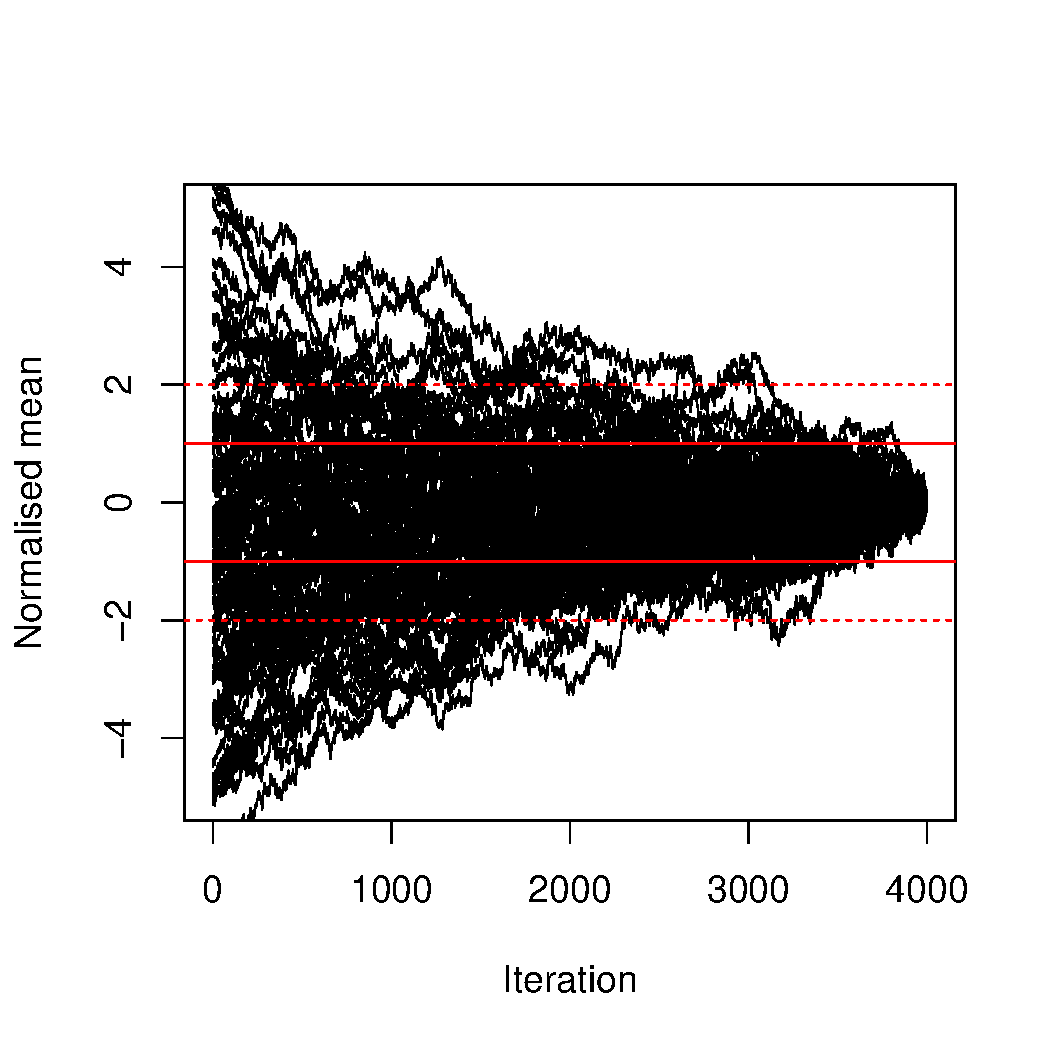
\includegraphics{figs/AllMeanParticles.pdf}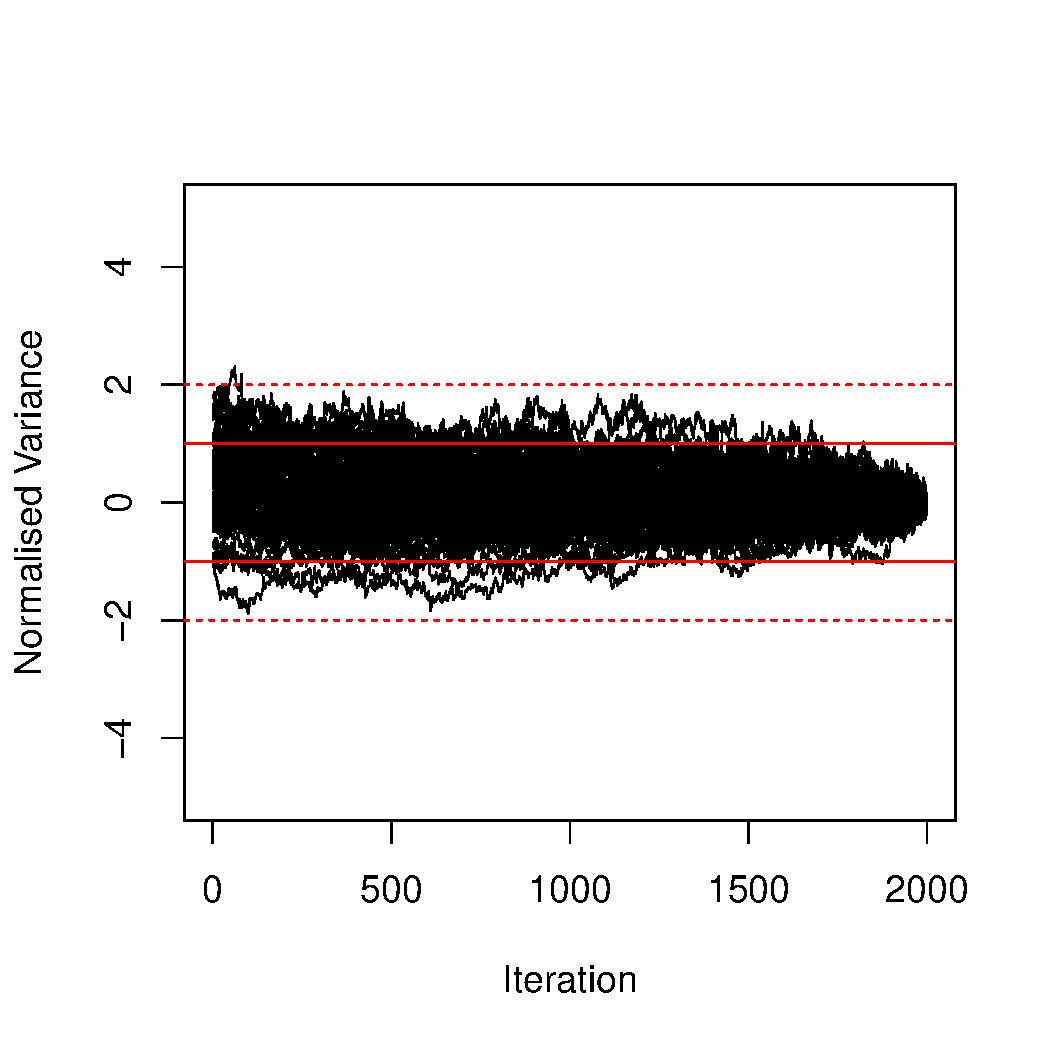
\includegraphics[]{figs/AllVarParticles.pdf}}
\caption{Normalised mean (left panel) and variance (right panel) of each parameter in our model, as functions of iterations. The normalisation values are the mean and variance of the ensemble of particles positions at the last iteration. Red lines show one and two sigma levels of these normalisation values.}
\label{convergence}
\end{center}
\end{figure*}

Once all parameters have entered the equilibrium state, we stop \emph{emcee} sampling using the criterium of \citet{Gong2016} \footnote{Implemented in the R package \emph{mcmcse} \citep{mcmcse}}. We chose this criterium because it was developed for high-dimensional problems and tested on Hierarchical Bayesian Models. In this criterium, the MCMC chain stops once its "effective sample size" (ESS, the size that an independent and identically distributed sample must have to provide the same inference) is larger than a minimum sample size computed using the required accuracy, $\upsilon$, for each parameter confidence interval $(1-\delta)$100\%. Our \emph{emcee} run stops once the ESS of the ensemble of walkers is greater than the minimum sample size needed for the required accuracy $\epsilon = 0.05$ on the 68\% confidence interval ($\delta = 0.32$) of each parameter.


\section{Codes}
\label{sect:code}
This Section sets out the details about the code I develop to perform the computation described throughout this chapter. First, I give a brief chronological description of the model development. Later, I will describe the details on the implementation of the charged PSO, the modified \emph{emcee}, and the GMM used to describe the field population. Finally, I will end this Section detailing the hybrid high performance computing code developed to minimise the computing time of the BHM.

The first version of the Bayesian Hierarchical Model was implemented by \'Angel Berihuete in the package \emph{Stan} \citep{Stan}. It comprised a Bayesian model of the ML model of \citet{Sarro2014}. The proper motions were modelled using a single mixture of gaussians. The photometry was modelled with a Chebyshev polynomial parametrised with the length along the sequence. This length was found using a principal curve analysis. Later, I included the EMB and uncertainties both in proper motion and in photometry, and the width of the sequence modelled as the multivariate gaussian. We realised that the principal curve analysis is not compatible with the deconvolution methodology. The principal curve analysis is driven by the elements with higher variance. We decided to parametrise the polynomials with the true colour, a nuisance parameter that was marginalised with the aid of a prior. For this prior we introduced the colour distribution. Previous to the introduction of the marginalisation of the nuisance parameters, the model worked fine on samples of a few thousands of stars. One the marginalisation was introduced the model increased the amount of computing time rendering it useless for higher data sizes. At this point we decided to port the existing code into python in order to use the parallel \emph{emcee}. \emph{emcee} proved to be of great use. Due to its parallelisation capabilities we were able to increase the data size from 2000 to 10,000 objects. Since the computing of the likelihood was the highest computational challenge, I developed my own routines to perform it on parallel. However, \emph{CosmoHammer} \citep{Akeret2013} turn out to be more efficient in distributing the loads. I ported the code into \emph{CosmoHammer} and modified this last one to better suit our needs. Despite the Hybrid-HPC, the computing of the likelihood of $10^5$ seemed unreachable. At this point I performed two tasks, the first was to strip the code of all auxiliary libraries calls, and the vectorisation of the operations. Since the parameters of the field were held fixed, the field likelihood was computed externally for each object. The code was then fed with the data, the field likelihood, and the auxiliary computations reduced at minimum. These reduction included for example, the Cholesky decompositions and matrix inversions of the uncertainty. Thus, instead of doing these computation inside the code, the code was fed with the appropriate values.

Introducing PSO and later the charged PSO reduced the computing time.  At this point we were able to compute the first $10^5$ run, which however did not converged in reasonable time. Once the approximation to the marginalisation integrals (Eqs. \ref{eq:clmarginalps} and \ref{eq:clmarginalpb}) were introduced, the computing time reduced far more. Finally, the tuning of the parameter allowed us to increase the acceptance fraction, and reach convergence within 4 weeks of full computing time in a 80 cores computer cluster. It is indeed a very long time, however it is reasonable compared with our original estimates of approximately 2 years\footnote{Today, the DANCe team is working on a GPU version of the code which is expected to compute the same amount of calculations in a couple of days.}.

\subsection{The modified charged PSO}
\label{sect:chargedPSO}
As explained before, the charged PSO of \citet{Blackwell2002} was inappropriate to our objective. The metric of the parametric space of our problem is not isotropic, parameters have different length scales. For example, while fraction are constrained in the $[0,1]$ interval proper motions parameters can go far larger than that. Therefore, the use of an isotropic metric results in a solution which is crowded in some parameters while is over dispersed in others. 
To solve this issue, I modified the charged PSO by measuring distance between particles and applying the electrostatic force independently in each parameter. In such a way, the electrostatic force plays a role only when the relative distance between particles is smaller than $10^{-10}$. I found this value heuristically.

In the original version of  \citet{Blackwell2002}, each particle is subject to the acceleration,
\begin{equation}
\label{eq:PSOacc}
\mathbf{a}=\sum_{i\neq j} \frac{q_i \cdot q_j }{r_{ij}^3} \cdot \mathbf{r}_{ij}, \ \ \ \ p_{core} < r_{ij} < p
\end{equation}
where $q_i$ and $q_j$ are the charges of particles $i$ and $j$, $r_{ij}$ is the distance between them. The distances $p_{core}$ and $p$ indicate the minimum and maximum distances at which the electrostatic force came into action. Outside this range, the electrostatic force is zero. In this equation, $\mathbf{r}_{ij}= \mathbf{x}_i -\mathbf{x}_j$, where $\mathbf{x}_i,\mathbf{x}_j$ are the positions of particles $i$ and $j$. Also, $\mathbf{r}_{ij},\mathbf{x}_i,\mathbf{x}_j \subset \mathbb{R}^d$, with $d$ the dimension of the space. 

In the modified version, the distance is measured independently in each dimension of the parametric space. Thus, $\mathbf{r}_{ij}= \{x_{1,i} -x_{1,j},x_{2,i} -x_{2,j},...,x_{d,i} -x_{d,j}\}$. Also the acceleration has the form,
\begin{equation}
\label{eq:PSOacc}
\mathbf{a}=\sum_{i\neq j} \frac{q_i \cdot q_j }{r_{ij}^2} \cdot \mathbf{r}_{ij}, \ \ \ \  10^{-50} < \frac{r_{ij}}{r_{eq}} < \epsilon
\end{equation}
and it is now applied over each dimension of the parametric space. The distance $r_{eq}$ is that at which the velocity caused by the acceleration equals the mean velocity caused by the common PSO. $\epsilon$ is a free parameter set, heuristically, to $10^{-10}$.

\subsection{Improvements of emcee}
The modification I introduced in \emph{emcee}, although very simple, improved the acceptance fraction and mixing of the particles.
To allow the parallelisation, \citet{Foreman2013} divide the ensemble of particles in two ensembles. In the original version, the particles in one ensemble use one and the same particle in complementary ensemble to compute their positions according to Eq. \ref{eq:stretchmove}. In the modified versions, particles from one ensemble update their positions using a particle from the complementary ensemble, however, this particle is chosen randomly at each iteration. 

Figure \ref{fig:emceeDANCe} compares the mixing and acceptance fractions of the original and modified versions of \emph{emcee}. In a private communication with David Foreman, he mentioned that a similar modification was already introduced in a beta version of \emph{emcee}.
\begin{figure}[htbp]
\begin{center}
%\includegraphics[width=\textwidth]{}
\caption{Comparison between the log posterior evaluations of the original emcee version (left) and the modified one (right). }
\label{fig:emceeDANCe}
\end{center}
\end{figure}
\subsection{GMM for the field population}
As mentioned earlier in this Chapter, the field population is modelled by means of two independent photometric and proper motion distributions. The MLE of the parameters of these distributions were found using the EM algorithm.  The conventional EM algorithm for GMM \citep{Dempster1977} for a mixture of $M$ gaussians goes as follows. Given a set of parameters $\theta=\{w_i,\boldsymbol{\mu}_i,\boldsymbol{\Sigma}_i\}_{i=1}^M$, were $w_i$,$\boldsymbol{\mu}_i$, and $\boldsymbol{\Sigma}_i$ are the fraction, mean and covariance matrix of gaussian component $i$, the likelihood of the data is,

\begin{equation}
p(\{\mathbf{y}_n\}_{n=1}^N|\theta)=\prod_{n=1}^N {\sum_{i=1} ^M {w_i\cdot \mathcal{N}(\mathbf{y}_n|\boldsymbol{\mu}_i,\boldsymbol{\Sigma}_i)}}.
\end{equation}

To solve the problem, the EM algorithm requires  a set of $N$ variables, $z$, of $M$ dimension are introduced. The variable $z_{n,i}$ represent the probability that observation $y_n$ was drawn from gaussian $i$. Therefore,

\begin{equation}
1=\sum_{i=1}^M z_{n,i}
\end{equation}

These $z$ latent variables are found as
\begin{equation}
z_{n,i}= \frac{w_i\cdot \mathcal{N}(\mathbf{y}_n|\boldsymbol{\mu}_i,\boldsymbol{\Sigma}_i)}{\sum_{i=1}^M w_i\cdot \mathcal{N}(\mathbf{y}_n|\boldsymbol{\mu}_i,\boldsymbol{\Sigma}_i)}
\end{equation}

The EM works, as its name indicates, by maximising the expected value of the likelihood.
\begin{equation}
E[p(\{\mathbf{y}_n\}_{n=1}^N|\theta)]=\prod_{n=1}^N {\sum_{i=1} ^M {z_{n,i}\cdot w_i\cdot \mathcal{N}(\mathbf{y}_n|\boldsymbol{\mu}_i,\boldsymbol{\Sigma}_i)}}.
\end{equation}

The previous expectation is maximal when,
\begin{align}
w_i &= \frac{1}{N} \sum_{n=1}^N z_{n,i}, \\
\boldsymbol{\mu}_i &= \frac{1}{\sum_{n=1}^N z_{n,i}} \sum_{n=1}^N z_{n,i}\cdot \mathbf{y}_n\\
\boldsymbol{\Sigma}_i &= \frac{1}{\sum_{n=1}^N z_{n,i}} \sum_{n=1}^N z_{n,i}\cdot (\mathbf{y}_n - \boldsymbol{\mu}_i)\times(\mathbf{y}_n-\boldsymbol{\mu}_i)^T
\end{align}

The modified version of the GMM, which includes a uniform distribution, is now a particular case of the GMM. This can be viewed as a gaussian distribution with fixed parameters and a constant probability $c$ given by the uniform distribution. The new expectation is then,
\begin{equation}
E[p(\{\mathbf{y}_n\}_{n=1}^N|\theta)]=\prod_{n=1}^N {\left[z_{n,0}\cdot w_0 \cdot c + \sum_{i=1} ^M {z_{n,i}\cdot w_i\cdot \mathcal{N}(\mathbf{y}_n|\boldsymbol{\mu}_i,\boldsymbol{\Sigma}_i)}\right]}.
\end{equation}

The maximisation step remains identical except for the indices. There are now $M+1$ fractions $w_i$, with $i=0,1,...,M$, and the means and covariances run from $i=1,...,M$.

Regarding the photometric GMM of the field. Since photometry has missing values, we use the EM algorithm of \citet{McMichael1996}. This algorithm was developed to obtain the MLE of data with missing values. A more recent version has been developed by \citet{Lin2006}, however, this assumes that the missing data is randomly distributed (missing at random). As mentioned earlier, the missing values in the photometry are not randomly distributed.

In \citet{McMichael1996} algorithm, there is a set of $N$ gain matrices, one for each datum. Each $M_n$ matrix is an identity matrix in which the rows of the corresponding missing value have been deleted. Thus, the expected value of the likelihood is now,

\begin{equation}
E[p(\{\mathbf{y}_n\}_{n=1}^N|\theta)]=\prod_{n=1}^N {\sum_{i=1} ^M {z_{n,i}\cdot w_i\cdot \mathcal{N}(\mathbf{y}_n|M_n \boldsymbol{\mu}_i,M_n\boldsymbol{\Sigma}_i M_n)}}.
\end{equation}

The maximisation step is now,

\begin{align}
w_i &= \frac{1}{N} \sum_{n=1}^N z_{n,i}, \\
\boldsymbol{\mu}_i &= \frac{ \sum_{n=1}^N z_{n,i}\cdot H_n \mathbf{y}_n}{\sum_{n=1}^N z_{n,i} H_n M_n}
\end{align}
with 
\begin{equation}
H_i=M_i^T(M\Sigma_i M^T)^{-1}
\end{equation}

The maximisation step has no analytical solution for the covariance matrix, therefore, a modified steepest descent is used

\begin{equation}
\Sigma_i \leftarrow \Sigma_i + \frac{\rho}{2}\cdot \Sigma_i\Delta_i\Sigma_i,
\end{equation}
with  and $\Delta_i$ given by

\begin{equation}
\Delta_i=  \frac{1}{\sum_{n=1}^N z_{n,i}}\cdot \sum_{n=1}^N z_{n,i} \cdot \left[H_n(\mathbf{y}_n -  M_n \boldsymbol{\mu}_i) \times  (\mathbf{y}_n -  M_n \boldsymbol{\mu}_i)^TH_n^T - H_nI\right]
\end{equation}
 
 The algorithm preserves the monotonic convergence of the conventional EM, and returns positive definite matrices provided that $\rho < 2$. For details and validation see \citet{McMichael1996}.

\subsection{Hybrid-HPC implementations}
\label{sect:HHPC}
As I outlined at the beginning of this section, the parallel computing approach was an unavoidable step. Once the code was ported to python and \emph{CosmoHammer}, I modified this last one to better fit our needs. The modifications were mainly on the management of input and output files and the python \emph{multiprocessing} package for the computing of our likelihood. Also, I striped some of its original functions to reduce memory usage and implemented some others, like the use of initial positions for the particles.

In our Hybrid-HPC (HHPC) approach, the particles of \emph{emcee} are distributed on the nodes of the computing cluster. Then, each core in the node computes the likelihood of one fraction of the objects in the data set. For the cluster at the Centre of Astrobiology
\footnote{Villanueva de la ca\~nada, Madrid,Spain.}(CAB) I used a configuration of 6 nodes each with 12 cores. For the cluster at the University of C\'adiz, I used a configuration of 5 nodes each with 16 cores. Particles were distributed among the six nodes using MPI while each core computes the likelihood of one 12th of the total number of objects in the data set.

However, the HHPC approach was not the best solution at the CIMENT clusters of the University of Grenoble Alpes. At this cluster (Froggy) the HHPC continuously render errors of communication. For this reason, I implemented a only MPI version of the code. In this version, the multithreading approach is left aside. Instead, the totality of the available cores is fully dedicated to the computing of the likelihood. Each of the $n$ cores computes the likelihood of one $n$th of the objects in the data set. Once the likelihood of all particles has been computed, the master evaluates the new positions of the particles.

I finish this chapter with a brief description of the difficulties faced on the development and testing of the BHM code. As the code evolved in complexity, my computational skills were compelled to evolve as well. I started by learning R and solving some toy problems on it. Later, when the dimensionality of the posterior increased I learned \emph{Stan}. When the data set increased in size, we faced the parallelisation, so I learned Python and MPI. Once these versions were operable, I was forced to deal with libraries, from the common, numpy, scipy and numba, to the linking of modules and libraries. Finally, when dealing with several clusters I learned the queue languages Condor, slurm and OAR. Currently, the DANCe team has developed a GPU implementation of the BHM code.  



